\chapter{O LIMITE DE UMA FUNÇÂO}
\label{cap:limfunc}
\quad O estudo de limite de uma função visa determinar o que acontece (estudo do comportamento) com valores da imagem da função quando, no domínio dessa função, toma-se valores suficientemente próximos de um determinado ponto (número).\\

\section{Definição intuitiva de Limite de uma função}
De acordo com \citeonline[p. 93]{stewart} escrevemos $$\lim_{x \to a} f(x) = L$$
e dizemos "  o limite de $f(x)$, quando $x$ tende a $a$, é igual a $L$ " \quad  se pudermos tornar os valores de $f(x)$ arbitrariamente próximos de $L$ (tão próximos de $L$ quanto quisermos), tornando $x$ suficiente próximo de $a$ (por ambos os lados de $a$) mas não igual a $a$.\\

Em outras palavras, isso significa que a existência de um limite de uma função, quando $x$ tende a $a$, não depende necessariamente que a função esteja definida no ponto $a$ pois quando calculamos um limite, considera-se os valores da função tão próximos quanto se queira do ponto $a$, porém diferente de $a$, ou seja, considera-se os valores da função na vizinhança do ponto $a$.\\


Deve-se prestar atenção quando se diz que $x \neq a$ na definição de limite, ou seja, significa que ao procurar o limite de $f(x)$ quando $x$ tende a $a$ nunca consideramos $x=a$. Na verdade, $f(x)$ não precisa sequer estar definida quando $x=a$. A única coisa que importa é como $f$ está definida próximo de $a$ \cite[p.93]{stewart}.\\

 Considere  a função dada por Leithold (1994, p.56) definida por $\displaystyle f(x) = \frac{2x^2+x-3}{x-1}$ com $x \in \mathbb{R}$ e $x \neq 1$. Estudando o limite de $f(x)$ quando  $x$ tende a $1$, ou seja: 
$ \displaystyle \lim_{x \to 1} f(x) $.


\quad Observe que para  $x=1$, a função não é definida, ou seja, não existe o $f(1)$, pois\\

$$ \displaystyle
\lim_{x \to 1} f(x)= \lim_{x \to 1} \frac{2x^2+x-3}{x-1} = \frac{2 . 1^2+1-3}{1-1} = \frac{0}{0}
$$
resultando numa indeterminação, logo para solucionar esta indeterminação fatoramos o numerador obtendo:


$$ \displaystyle
f(x) = \frac{2x^2+x-3}{x-1} = \frac{(2x+3)(x-1)}{x-1} = 2x + 3
$$\\
\begin{citacao}
Conforme \citeonline[p. 69]{leithold}, se $x \neq 1$, o numerador e o denominador podem ser divididos por $(x-1)$ para obtermos $2x+3$. Lembre-se que quando calculamos o limite de uma função, à medida que $x$ aproxima-se de  1, estamos considerando valores de $x$ próximos a 1 mas não iguais a 1. Portanto é possível dividir o numerador e o denominador por $x-1$.
\end{citacao}
Logo, simplificando a expressão, tem-se:\\

$$
\displaystyle \lim_{x \to 1}f(x) = \lim_{x \to 1} \frac{2x^2+x-3}{x-1} = \lim_{x \to 1} \frac{(2x+3)(x-1)}{(x-1)} = \lim_{x \to  1} 2x+3 = 2 + 3 = 5
$$\\

Portanto, mesmo não existindo $f(1)$, o limite de $f(x)$ quando $x$ tende a 1 existe.

\begin{figure}[H]
\centering % para centralizarmos a figura
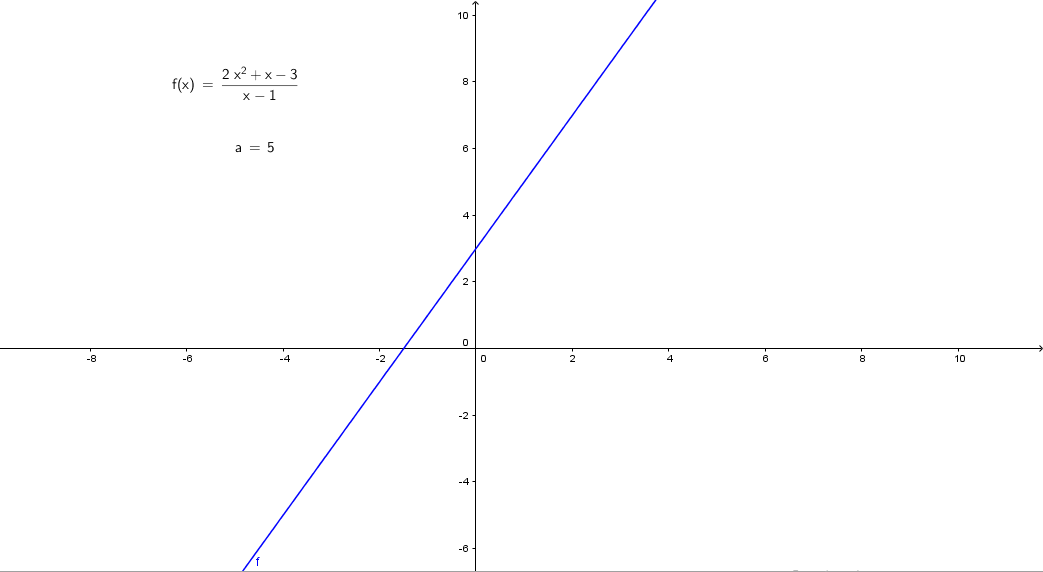
\includegraphics[width=15cm]{img/sub11.png} % leia abaixo
\caption{Gráfico de $f(x)$}
\label{fig:graph2}
\end{figure}

Analisando intuitivamente a função $f$ quando $x$  assume valores próximos de $1$, porém diferente de $1$. Atribuindo a $x$ valores próximos de $1$, porém menores que $1$, tem-se:

\begin{table}[H]
\centering
\caption{Tabela de valores para $f(x) = 2x+3$}
\label{tab:tab1}
\smallskip
\begin{tabular}{l|l|l|l|l|l|l|l|l}
\hline
 $x$ & $0$ & $0,25$ & $0,5$ & 0,75& $0,9$& $0,99$ & $0,999$ & $0,9999$\\[0.5ex]
\hline
&&&&&&&&\\[-2ex]
$f(x) = 2x+3$ & $3$ &  $3,5$ &  $4$ &  $4,5$ &  $4,8$&  $4,98$ &  $4,998$ &  $4,9998$\\[0.5ex]
\hline
\end{tabular}
\end{table}
Atribuindo a $x$ valores próximos de $1$, porém maiores que $1$, tem-se:
\begin{table}[H]
\centering
\caption{Tabela de valores para $f(x) = 2x+3$}
\label{tab:tab20}
\smallskip
\begin{tabular}{l|l|l|l|l|l|l|l|l}
\hline
 $x$ & $2$ & $1,75$ & $1,5$ & 1,25& $1,1$& $1,01$ & $1,001$ & $1,0001$\\[0.5ex]
\hline
&&&&&&&&\\[-2ex]
$f(x) = 2x+3$ & $7$ &  $6,5$ &  $6$ &  $5,5$ &  $5,2$&  $5,02$ &  $5,002$ &  $5,0002$\\[0.5ex]
\hline
\end{tabular}
\end{table}
Observa-se em ambas as tabelas que, à medida que $x$ se aproxima cada vez mais de 1, $f(x)$ torna-se cada vez mais próxima 5.\\
Nota-se na Tabela \ref{tab:tab1} que:\\
$ x = 0 \Rightarrow f(x) = 3 \quad \textrm{, isto é, } \quad x-1=0-1=-1\Rightarrow f(x) - 5 = 3-5 = -2$
$ x = 0,25 \Rightarrow f(x) = 3,5  \quad \textrm{, isto é, } \quad x-1=0,25-1=-0,75\Rightarrow f(x) - 5 = 3,5-5 = -1,5$
$ x = 0,5 \Rightarrow f(x) = 4 \quad \textrm{, isto é, } \quad x-1=0,5-1=-0,5\Rightarrow f(x) - 5 = 4-5 = -1$ \\
\vdots \\
$ x = 0,9999 \Rightarrow f(x) = 4,9998 \quad \textrm{, isto é, } \quad x-1=0,9999-1=-0,0001\Rightarrow f(x) - 5 = 4,9998-5 = -0,0002$\\
e, a Tabela \ref{tab:tab20}  mostra que:\\
$ x = 2 \Rightarrow f(x) = 7 \quad \textrm{, isto é, } \quad x-1=2-1=1\Rightarrow f(x) - 5 = 7-5 = 2$
$ x = 1,75 \Rightarrow f(x) = 6,5  \quad \textrm{, isto é, } \quad x-1=1,75-1=0,75\Rightarrow f(x) - 5 = 6,5-5 = 1,5$
$ x = 1,5 \Rightarrow f(x) = 6 \quad \textrm{, isto é, } \quad x-1=1,5-1=0,5\Rightarrow f(x) - 5 = 6-5 = 1$ \\
\vdots \\
$ x = 1,0001 \Rightarrow f(x) = 5,0002 \quad \textrm{, isto é, } \quad x-1=1,0001-1= 0,0001\Rightarrow f(x) - 5 = 5,0002-5 = 0,0002$\\
Portanto, pelas duas tabelas, \ref{tab:tab1} e \ref{tab:tab20}, tem-se que:\\
$
\vert x-1 \vert = 1 \Rightarrow \vert f(x) -5 \vert = 2 \\
\vert x-1 \vert = 0,75 \Rightarrow \vert f(x) -5 \vert = 1,5 \\
\vert x-1 \vert = 0,5 \Rightarrow \vert f(x) -5 \vert = 1 \\
\vdots \\
\vert x-1 \vert = 0,0001 \Rightarrow \vert f(x) -5 \vert = 0,0002 
$

Observa-se que se pode tomar $f(x)$ tão próximos de 5 quanto se deseja, bastando para isto tomar $x$  suficiente próximos de 1.\\

Outra forma mais precisa de dizer isto é que se pode tornar o valor absoluto da diferença entre $x$ e 1 suficiente  pequeno. Isto é, $|f(x)-5|$ pode se tornar tão pequeno quanto se desejar, tomando $|x-1|$ suficientemente pequeno.  A matemática utiliza as letras gregas $\epsilon$ (epsilon) e $\delta$ (delta) para indicar essas pequenas diferenças. Assim, dado um número $\varepsilon$, podemos  tornar $\vert f(x) - 5\vert < \varepsilon$ onde, calculando o módulo, resulta:
$$1 - \delta < x < 1 + \delta \Rightarrow 5 - \varepsilon < f(x) < 5 + \varepsilon$$\\
É importante perceber que $\delta$ depende do $\epsilon$ considerado. Nas duas tabelas tem-se que:

$$
\vert x - 1 \vert = 1 \Rightarrow \vert  f(x) - 5 \vert = 2
$$\\
Então; se dado $\epsilon = 2$, toma-se $\delta = 1$ e afirma-se que: $$0 < \vert x -1 \vert < 1 \Rightarrow \vert f(x) - 5 \vert < 2$$
onde calculando o módulo, resulta:
$$1 - 1 < x < 1+1 \Rightarrow 5 -2 < f(x) < 5+2$$
$$0 < x < 2 \Rightarrow 3 < f(x) < 7 $$
%%grafico
\begin{figure}[H]
\centering % para centralizarmos a figura
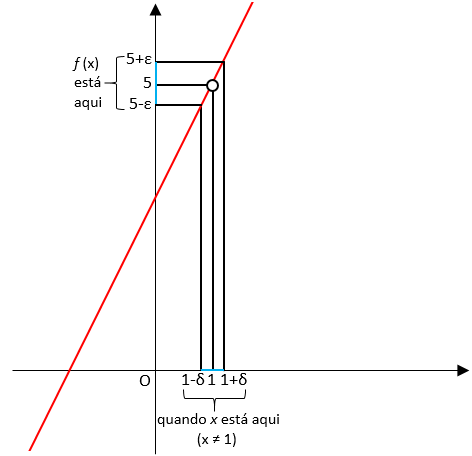
\includegraphics[width=10cm]{img/img2.png} % leia abaixo
\caption{Gráfico de $f(x)$}
\label{fig:img2}
\end{figure}



Desde que, para qualquer valor positivo de $\epsilon$, pode-se encontrar  um valor apropriado para $\delta$ tal que:
$$
0 < \vert x - 1 \vert < \delta \Rightarrow \vert f(x-5) \vert < \epsilon
$$
portanto se diz que  o limite de $f(x)$, para $x$ tendendo a 1, é 5, notado por:
$$
\lim_{x \to 1}  f(x) = 5
$$


\section{Definição Formal de Limite}
\quad Segundo Stewart (2009, p. 115) seja $f$ uma função definida sobre algum intervalo aberto que contém o número $a$, exceto possivelmente no próprio $a$. Então dizemos que o limite de $f(x)$ quando $x$ tende a $a$ é $L$, e escrevemos:
$$
\lim_{x \to a} f(x) = L
$$
se para todo número $\epsilon > 0$ há um número correspondente $\delta > 0$ tal que  $\vert f(x) - L \vert < \epsilon $ sempre que $0 < \vert x- a \vert < \delta$.\\

Nota-se de acordo com o exemplo abaixo que quando a função é determinada num ponto o $\displaystyle \lim_{x \to a} f(x) = f(a)$, mas quando a função não for determinada, ou seja, representada por uma das formas indeterminadas apresentadas no capítulo \ref{cap:indet}, que neste caso o conceito de limite se apresenta como alternativa para a abordagem adequada destas questões.\\

\textbf{Exemplo.} Seja a função $\displaystyle f(x) = \frac{x-2}{x^2-4}$, neste caso a função não esta definida para $x=2$, por isso que a definição de limite faz a diferença, pois ela aceita valores de $x$ que estão próximos de $a$, mas não iguais a $a$. Para resolver limites de funções indefinidas e indeterminadas pode-se lançar mão de resoluções por intuição, recursos algébricos ou mesmo geométricos.

\subsection{Resolução utilizando noção intuitiva}
Na resolução intuitiva constrói-se tabelas com valores se aproximando do ponto 2, uma com valores inferiores e outra com valores superiores, mas nunca igual a 2. Assim:

\begin{table}[H]
\centering
\label{tab:tabintuit}
\smallskip
\begin{tabular}{l|l|l|l|l}
 $x<2$ & $1,5$ & $1,9$ & $ 1,99$ & 1,999 \\[0.5ex]
\hline
&&&\\[-2ex]
$f(x)$ & $0,28$ &  $0,256$ &  $0,2506$ & 0,25006..\\[0.5ex]
\end{tabular}
\end{table}
ou
\begin{table}[H]
\centering
\label{tab:tabintuit}
\smallskip
\begin{tabular}{l|l|l|l|l}
 $x>2$ & $2,5$ & $2,1$ & $2,01$ &  2,001 \\[0.5ex]
\hline
&&&\\[-2ex]
$f(x)$ & $0,222$ &  $0,2439$ &  $0,2493$ & 0,24994..\\[0.5ex]
\end{tabular}
\end{table}

Com base nestes valores pode-se intuir que $\displaystyle \lim_{x \to 2} \frac{x-2}{x^2-4} = \frac{1}{4}$.

\subsection{Resolução por recursos algébricos}
Neste caso tem-se a fatoração algébrica e os pressupostos matemáticos como principais recursos. No exemplo pode-se começar fatorando o denominador, assim:
$$
\lim_{x \to 2} \frac{x-2}{x^2-4} = \lim_{x \to 2} \frac{x-2}{(x^2 - 2^2)} = \lim_{x \to 2} \frac{(x-2)}{(x-2)(x+2)}
$$
\qquad Como  na fatoração encontra-se no denominador um termo igual  no denominador, mas no ponto $x=2$ ele representa uma indeterminação e considerando a definição de limite onde diz que $x$ pode assumir valores próximos a 2 mas não iguais a 2. Logo, pode-se dividir o numerador e o denominador por $x-2$, então:
$$
\lim_{x \to 2} \frac{1}{x+2} = \frac{1}{4}
$$

\subsection{Resolução utilizando recursos geométricos}
A resolução de problemas através de recursos geométricos podem ser feitos com a utilização de softwares matemáticos como o Geogebra utilizado neste trabalho. Com a inserção destes softwares educativos os alunos são motivados a desenvolver habilidades de visualização, interpretação e resolução de problemas, proporcionando-lhes a construção do próprio conhecimento.

\begin{figure}[H]
\centering % para centralizarmos a figura
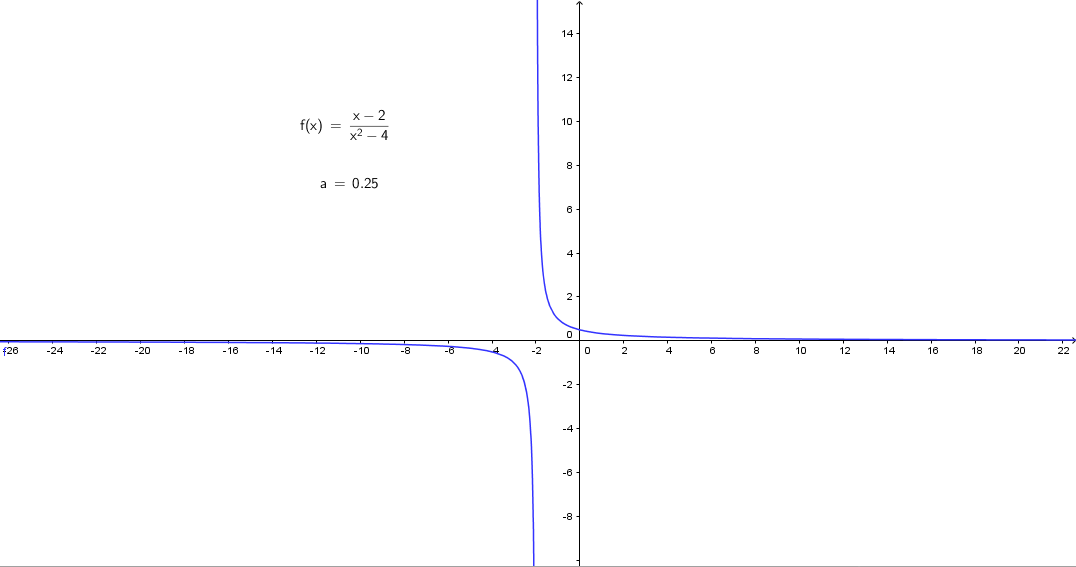
\includegraphics[width=15cm]{img/sub5.png} % leia abaixo
\caption{Gráfico de $f(x)$}
\label{fig:graph3}
\end{figure}


\section{Formas Indefinidas do Tipo $\displaystyle \frac{k}{0}$ que podem ser resolvidas com o uso de limites}

De acordo com o  item \ref{sec:expindk0}  a expressão $\displaystyle \frac{k}{0}$ é indefinida. Porém, a divisão $\displaystyle \frac{k}{0}$  pode ser contornada em se tratando de limites, ou seja, esta divisão pode ser infinita aplicando-se valores aos quocientes próximos a zero. Considerando  $k=1$ tem-se:\\
$
\displaystyle \frac{1}{0,1} = 10   \\
\displaystyle \frac{1}{0,01} = 100 \\ 
\displaystyle \frac{1}{0,001} =1000  \\
\displaystyle \frac{1}{0,0001} =10000  \\
\displaystyle \frac{1}{0,00001} = 100000 \\
\vdots \\
\displaystyle \frac{1}{0,0000000000001} = \textrm{número muito grande}   
$\\
%\end{array} 
%\end{displaymath}



Nota-se que quanto mais próximo o denominador de zero, maior é o valor da divisão tendendo ao infinito. Portanto, embora  $\displaystyle \frac{1}{0}$  seja indefinido no conjunto dos números, ficaria definido no cálculo de limites através do objeto numérico infinito. É importante destacar que o infinito não é um número real, não podendo ser realizadas determinadas operações aritméticas, as quais levariam a resultados absurdos e contraditórios.

\textbf{Teorema 1}
(Limites infinitos com $x \to 0^+$ ou $x \to 0^-$). Segundo Leithold (1994, p. 80) se $r$ for um inteiro positivo qualquer, então:\\
\textit{i) $\displaystyle \lim_{x \to 0^+} \frac{1}{x^r} = + \infty$\\
ii) $\displaystyle \lim_{x \to 0^-} \frac{1}{x^r} = - \infty \quad\textrm{se $r$ for ímpar} $\\
iii) $\displaystyle \lim_{x \to 0^-} \frac{1}{x^r} = + \infty \quad \textrm{se $r$ for par}$}\\


\textbf{Exemplo 1} Seja $\displaystyle f(x) = \frac{1}{x^2}$, com $x \neq 0$. Verificando os valores de $f(x)$ quando $x$ esta próximo de $0$.\\
Atribuindo a $x$ valores próximos de $0$, à esquerda de $0$, tem-se:

\begin{table}[H]
\centering
\caption{Tabela de valores para $\displaystyle f(x) = \frac{1}{x^2}$}
\label{tab:tab2}
\smallskip
\begin{tabular}{l|l|l|l}
\hline
 $x$ & $-0,1$ & $-0,01$ & $-0,001$ \\[0.5ex]
\hline
&&&\\[-2ex]
$f(x)$ & $100$ &  $10.000$ &  $1.000.000$\\[0.5ex]
\hline
\end{tabular}
\end{table}
Agora atribuindo a $x$ valores próximos  de $0$,  à direita de $0$, tem-se:

\begin{table}[H]
\centering
\caption{Tabela de valores para $\displaystyle f(x) = \frac{1}{x^2}$}
\label{tab:tab2}
\smallskip
\begin{tabular}{l|l|l|l}
\hline
 $x$ & $0,1$ & $0,01$ & $0,001$ \\[0.5ex]
\hline
&&&\\[-2ex]
$f(x)$ & $100$ &  $10.000$ &  $1.000.000$\\[0.5ex]
\hline
\end{tabular}
\end{table}

\textbf{Teorema 2}
(Limites Laterais). Segundo Leithold (1994, p. 74) \textit{  o limite de $f(x)$  existe e será igual a $L$ se e somente se $\displaystyle \lim_{x \to a^-} f(x)$ e $\displaystyle \lim_{x \to a^+} f(x)$ existirem e forem iguais.}\\

Nota-se que, quando $x$  se aproxima de $0$, quer pela esquerda ($x \to 0^-$), quer pela direita ($x \to 0^+$), $f(x)$ assume valores cada vez maiores (aumenta ilimitadamente). Logo, de acordo com o Teorema 2 pode-se escrever que:
$$
\displaystyle \lim_{x \to 0} f(x) = \lim_{x \to 0} \frac{1}{x^2} = + \infty
$$

Para melhor compreensão, observe o esboço do gráfico desta função na Figura \ref{fig:graph3}:\\
\begin{figure}[H]
\centering % para centralizarmos a figura
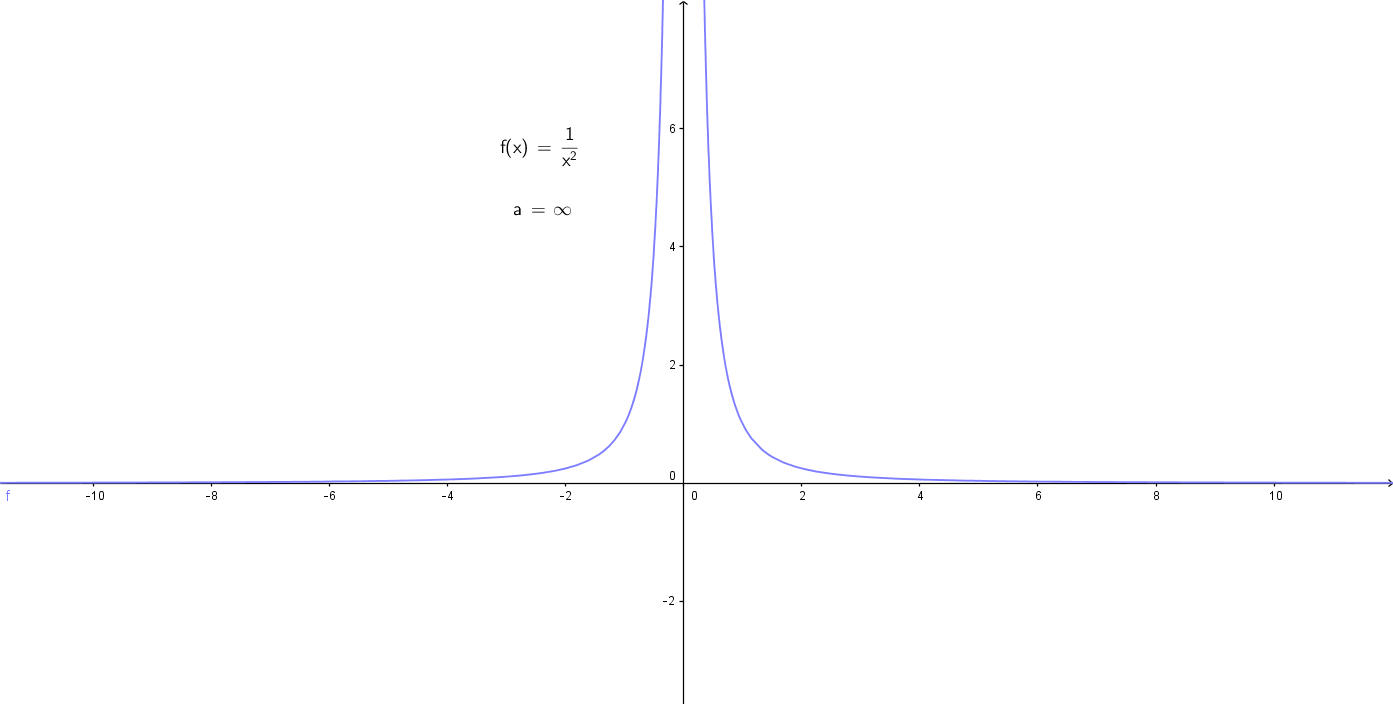
\includegraphics[width=15cm]{img/graph3.png} % leia abaixo
\caption{Gráfico de $f(x)$}
\label{fig:graph3}
\end{figure}

\textbf{Exemplo 2} Seja $f$ uma função $ \displaystyle f(x)=  - \frac{1}{x^2}$. De forma análoga, quando $x$ se aproxima de $0$, quer pela esquerda, quer pela direita, $f(x)$ assume valores cada vez menores (decresce ilimitadamente). Logo, pelo teorema dos limites laterais pode-se escrever:
$$
\lim_{x \to 0} f(x) = \lim_{x \to 0} - \frac{1}{x^2} = - \infty
$$\\

Para melhor compreensão, observe o comportamento de $f(x)$ tendendo ao infinito negativo, quando $x$ se aproxima de $0$.\\
\begin{figure}[H]
\centering % para centralizarmos a figura
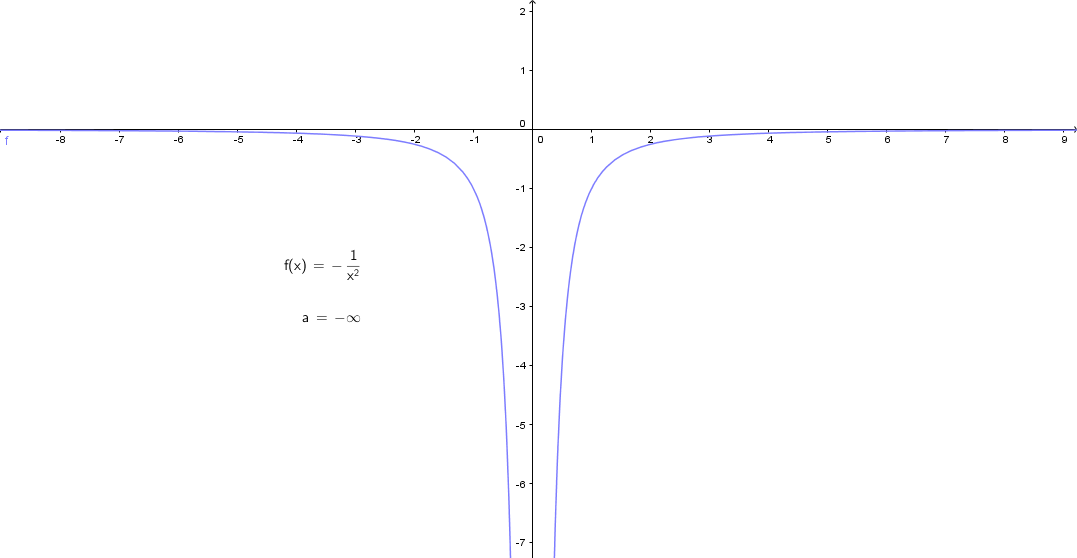
\includegraphics[width=15cm]{img/graph4.png} % leia abaixo
\caption{Gráfico de $f(x)$}
\label{fig:graph4}
\end{figure}

\quad Usa-se a notação $\displaystyle \lim_{x \to a} f(x) = + \infty$ ou $\displaystyle \lim_{x \to a} f(x) = - \infty$, contudo, o símbolo $\pm \infty$ não é considerado um número real, e portanto, não existe o limite, entretanto o símbolo indica que a função pode assumir valores tão grandes quanto quiser, bastando para isso escolhermos os valores de $x$ tão próximos de $a$ quanto se queira.\\

\textbf{Exemplo 3} Seja $\displaystyle f(x) = \frac{2x}{x-1}$, sendo $x \neq 1$


\begin{table}[H]
\centering
\caption{Tabela de valores para $\displaystyle f(x) = \frac{2x}{x-1}$}
\label{tab:tab2}
\smallskip
\begin{tabular}{l|l|l|l|l}
\hline
 $x$ & $1,1$ & $1,01$ & $1,001$ & $\to 1$ \\[0.5ex]
\hline
&&&&\\[-2ex]
$f(x)$ & $22$ &  $202$ &  $2002$& $\to + \infty$\\[0.5ex]
\hline
\end{tabular}
\end{table}

Observa-se que, quando $x$ tende a $1$ pela direita,  $f(x)$ assume valores positivos arbitrariamente grandes (aumenta ilimitadamente). Assim:
$$
\lim_{x \to 1^+} f(x) = \lim_{x \to 1^+} \frac{2x}{x-1} =  \frac{2}{0^+} = + \infty
$$


\begin{table}[H]
\centering
\caption{Tabela de valores para $\displaystyle f(x) = \frac{2x}{x-1}$}
\label{tab:tab2}
\smallskip
\begin{tabular}{l|l|l|l|l}
\hline
 $x$ & $0,9$ & $0,99$ & $0,999$ & $\to 1$ \\[0.5ex]
\hline
&&&&\\[-2ex]
$f(x)$ & $-18$ &  $-198$ &  $-1998$& $\to - \infty$\\[0.5ex]
\hline
\end{tabular}
\end{table}
Por outro lado, quando $x$ tende a $1$ pela esquerda, $f(x)$ assume valores cada vez menores (decresce ilimitadamente). Assim:
$$
\lim_{x \to 1^-} f(x) = \lim_{x \to 1^-}  \frac{2x}{x-1} = \frac{2}{0^-} = - \infty
$$
\begin{figure}[H]
\centering % para centralizarmos a figura
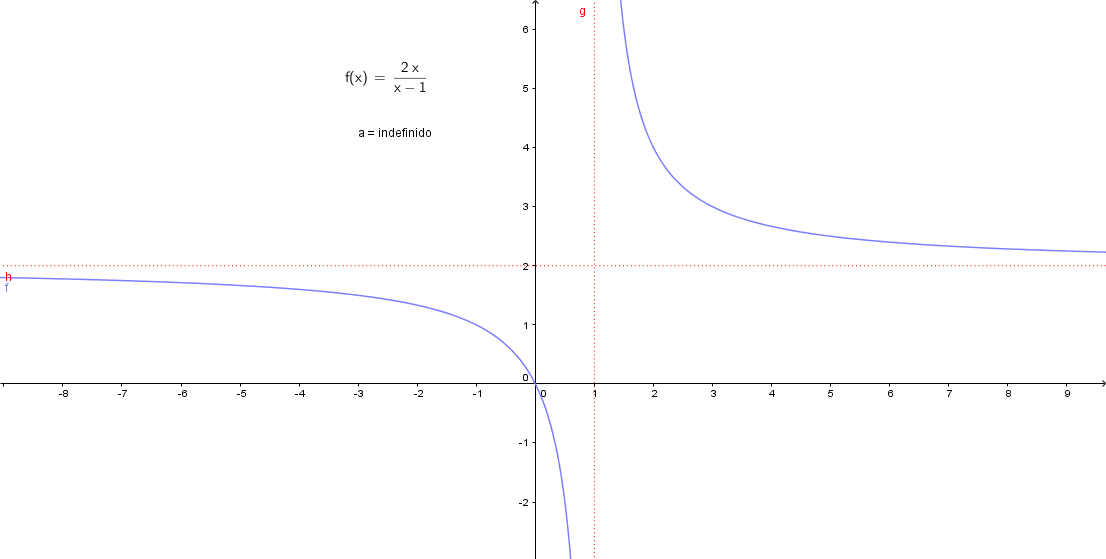
\includegraphics[width=15cm]{img/graph5.png} % leia abaixo
\caption{Gráfico de $f(x)$.}
\label{fig:graph5}
\end{figure}
Considerando a função $\displaystyle f(x) = \frac{2x}{x-1}$, exibida no gráfico da Figura \ref{fig:graph5}. A função aumenta sem limite quando $x$ tende a $1$ pela direita, mas decresce sem limite, à medida que $x$ se aproxima de $1$ pela esquerda. Assim, neste caso não há símbolo único para o limite bilateral neste caso. Dizemos que $\displaystyle \lim_{x \to 1} \frac{2x}{x-1}$ não existe.\\

\textbf{Teorema 3} (limite de uma função racional) Pode ser aplicado se $\displaystyle \lim_{x \to a} f(x) = 0$ e $\displaystyle \lim_{x \to a} g(x) = K$, onde $K$ é uma constante diferente de zero.\\

\textit{(i)} Se $K > 0$  e se $f(x) \to 0$ por valores positivos de $f(x)$,
$$
\lim_{x \to a} \frac{g(x)}{f(x)} = + \infty
$$

\textit{(ii)} Se $K > 0$  e se $f(x) \to 0$ por valores negativos de $f(x)$,
$$
\lim_{x \to a} \frac{g(x)}{f(x)} = - \infty
$$

\textit{(iii)} Se $K < 0$  e se $f(x) \to 0$ por valores positivos de $f(x)$,
$$
\lim_{x \to a} \frac{g(x)}{f(x)} = - \infty
$$

\textit{(iiii)} Se $K < 0$  e se $f(x) \to 0$ por valores negativos de $f(x)$,
$$
\lim_{x \to a} \frac{g(x)}{f(x)} = + \infty
$$
\quad O teorema será válido se "$x \to a$" for substituído por "$x \to a^+$" ou "$x \to a^-$". (Leithold, 1994, p. 81)\\

Aplicando esse terorema , pode-se frequentemente obter uma indicação de que o resultado será $+ \infty$ ou $- \infty$, tomando um valor adequado de $x$ próximo de $a$ para se assegurar de que o quociente é positivo ou negativo.



\section{As Formas Indeterminadas}
\quad Conforme \citeonline[p. 124]{stewart}, para o cálculo do limite de uma função quando $x$ tende a $a$ pode muitas vezes ser encontrado simplesmente calculando-se o valor da função em $a$. No entanto, algumas vezes esta regra falha. Isto acontece quando se faz a substituição direta de $x$ por seu valor de tendência e encontram-se indeterminações. É importante entender que, quando isso acontece, não se esta diante da resposta final. Neste caso, deve-se utilizar de artifícios algébricos para solucionar essas indeterminações.\\

\subsection{Forma do Tipo $\displaystyle \frac{0}{0}$}
\quad Se $f$ e $g$ forem duas funções tais que $\displaystyle \lim_{x \to a} f(x)= 0$ e $\displaystyle \lim_{x \to a} g(x)= 0$, então a função $\displaystyle \frac{f}{g}$ tem a forma indeterminada $\displaystyle \frac{0}{0}$ em $a$.\\

Essas situações acontecem frequentemente, logo para solucionar a indeterminação, se torna necessário o uso de técnicas de simplificação para calculá-las, como: fatoração, racionalização, dispositivo prático de Briot-ruffini para divisão de polinômios, etc.



\textbf{Exemplo 1} $$ \lim_{x \to 1} f(x) = \lim_{x \to 1} \frac{x^2 -1}{x-1} = \frac{1^2 - 1}{1-1} = \frac{0}{0} \quad \textrm{(indeterminação)}$$\\
Resolvendo o $$\lim_{x \to 1} f(x) =\lim_{x \to 1}  \frac{x^2-1}{x-1} = \lim_{x \to 1} \frac{(x+1)(x-1)}{(x-1)}$$

Como na definição de limite está pressuposto que $x$ pode ser próximo de $1$ mas nunca igual a $1$. Condição que se habilita fazer a simplificação, então:

$$\lim_{x \to 1} f(x) =\lim_{x \to 1} (x+1) = 1+ 1= 2$$
\begin{figure}[H]
\centering % para centralizarmos a figura
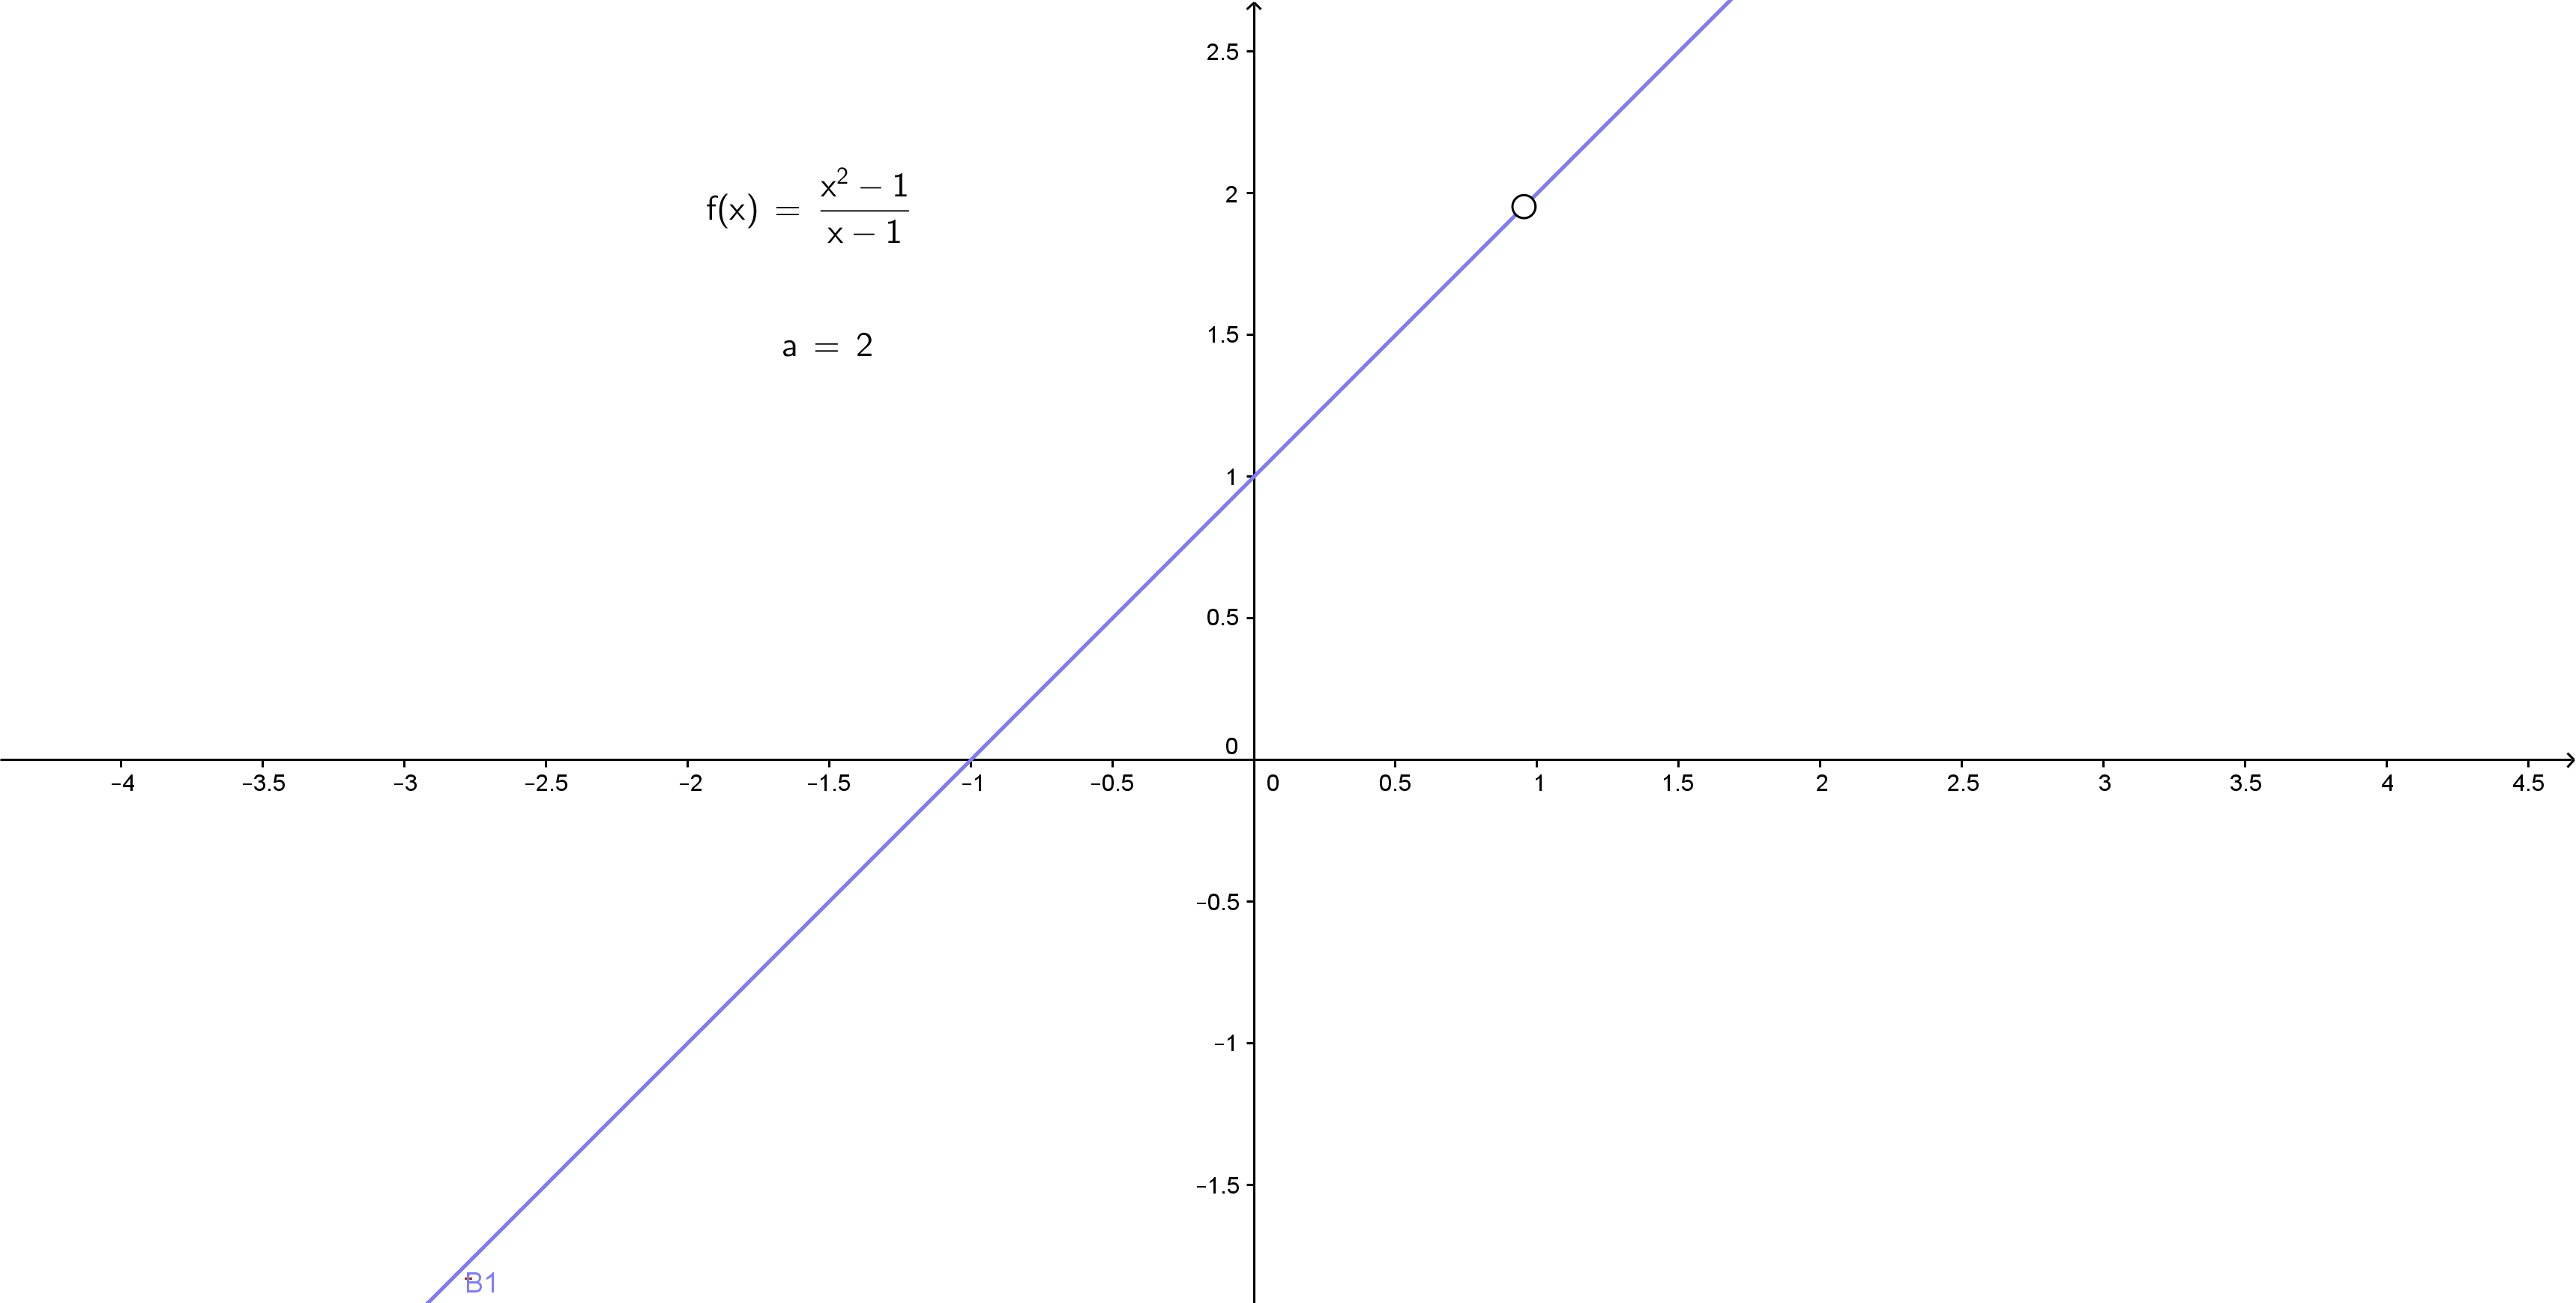
\includegraphics[width=15cm]{img/graph6.png} % leia abaixo
\caption{Gráfico de $f(x)$}
\label{fig:graph6}
\end{figure}

\textbf{Exemplo 2} $$\lim_{x \to 3} f(x) = \lim_{x \to 3} \frac{x^2-3x}{x-3}$$ Resolvendo o $$\displaystyle \lim_{x \to 3}  \frac{x^2-3x}{x-3} = \frac{3^2 - 3 . 3}{3-3}= \frac{0}{0} \quad \textrm{(indeterminação)}$$  Logo deve-se simplificar a expressão para solucionar a  indeterminação, então:
$$\lim_{x \to 3} \frac{x^2 - 3x}{x-3} = \lim_{x \to 3} \frac{x(x-3)}{x-3}= \lim_{x \to 3} x = 3$$\\

\begin{figure}[H]
\centering % para centralizarmos a figura
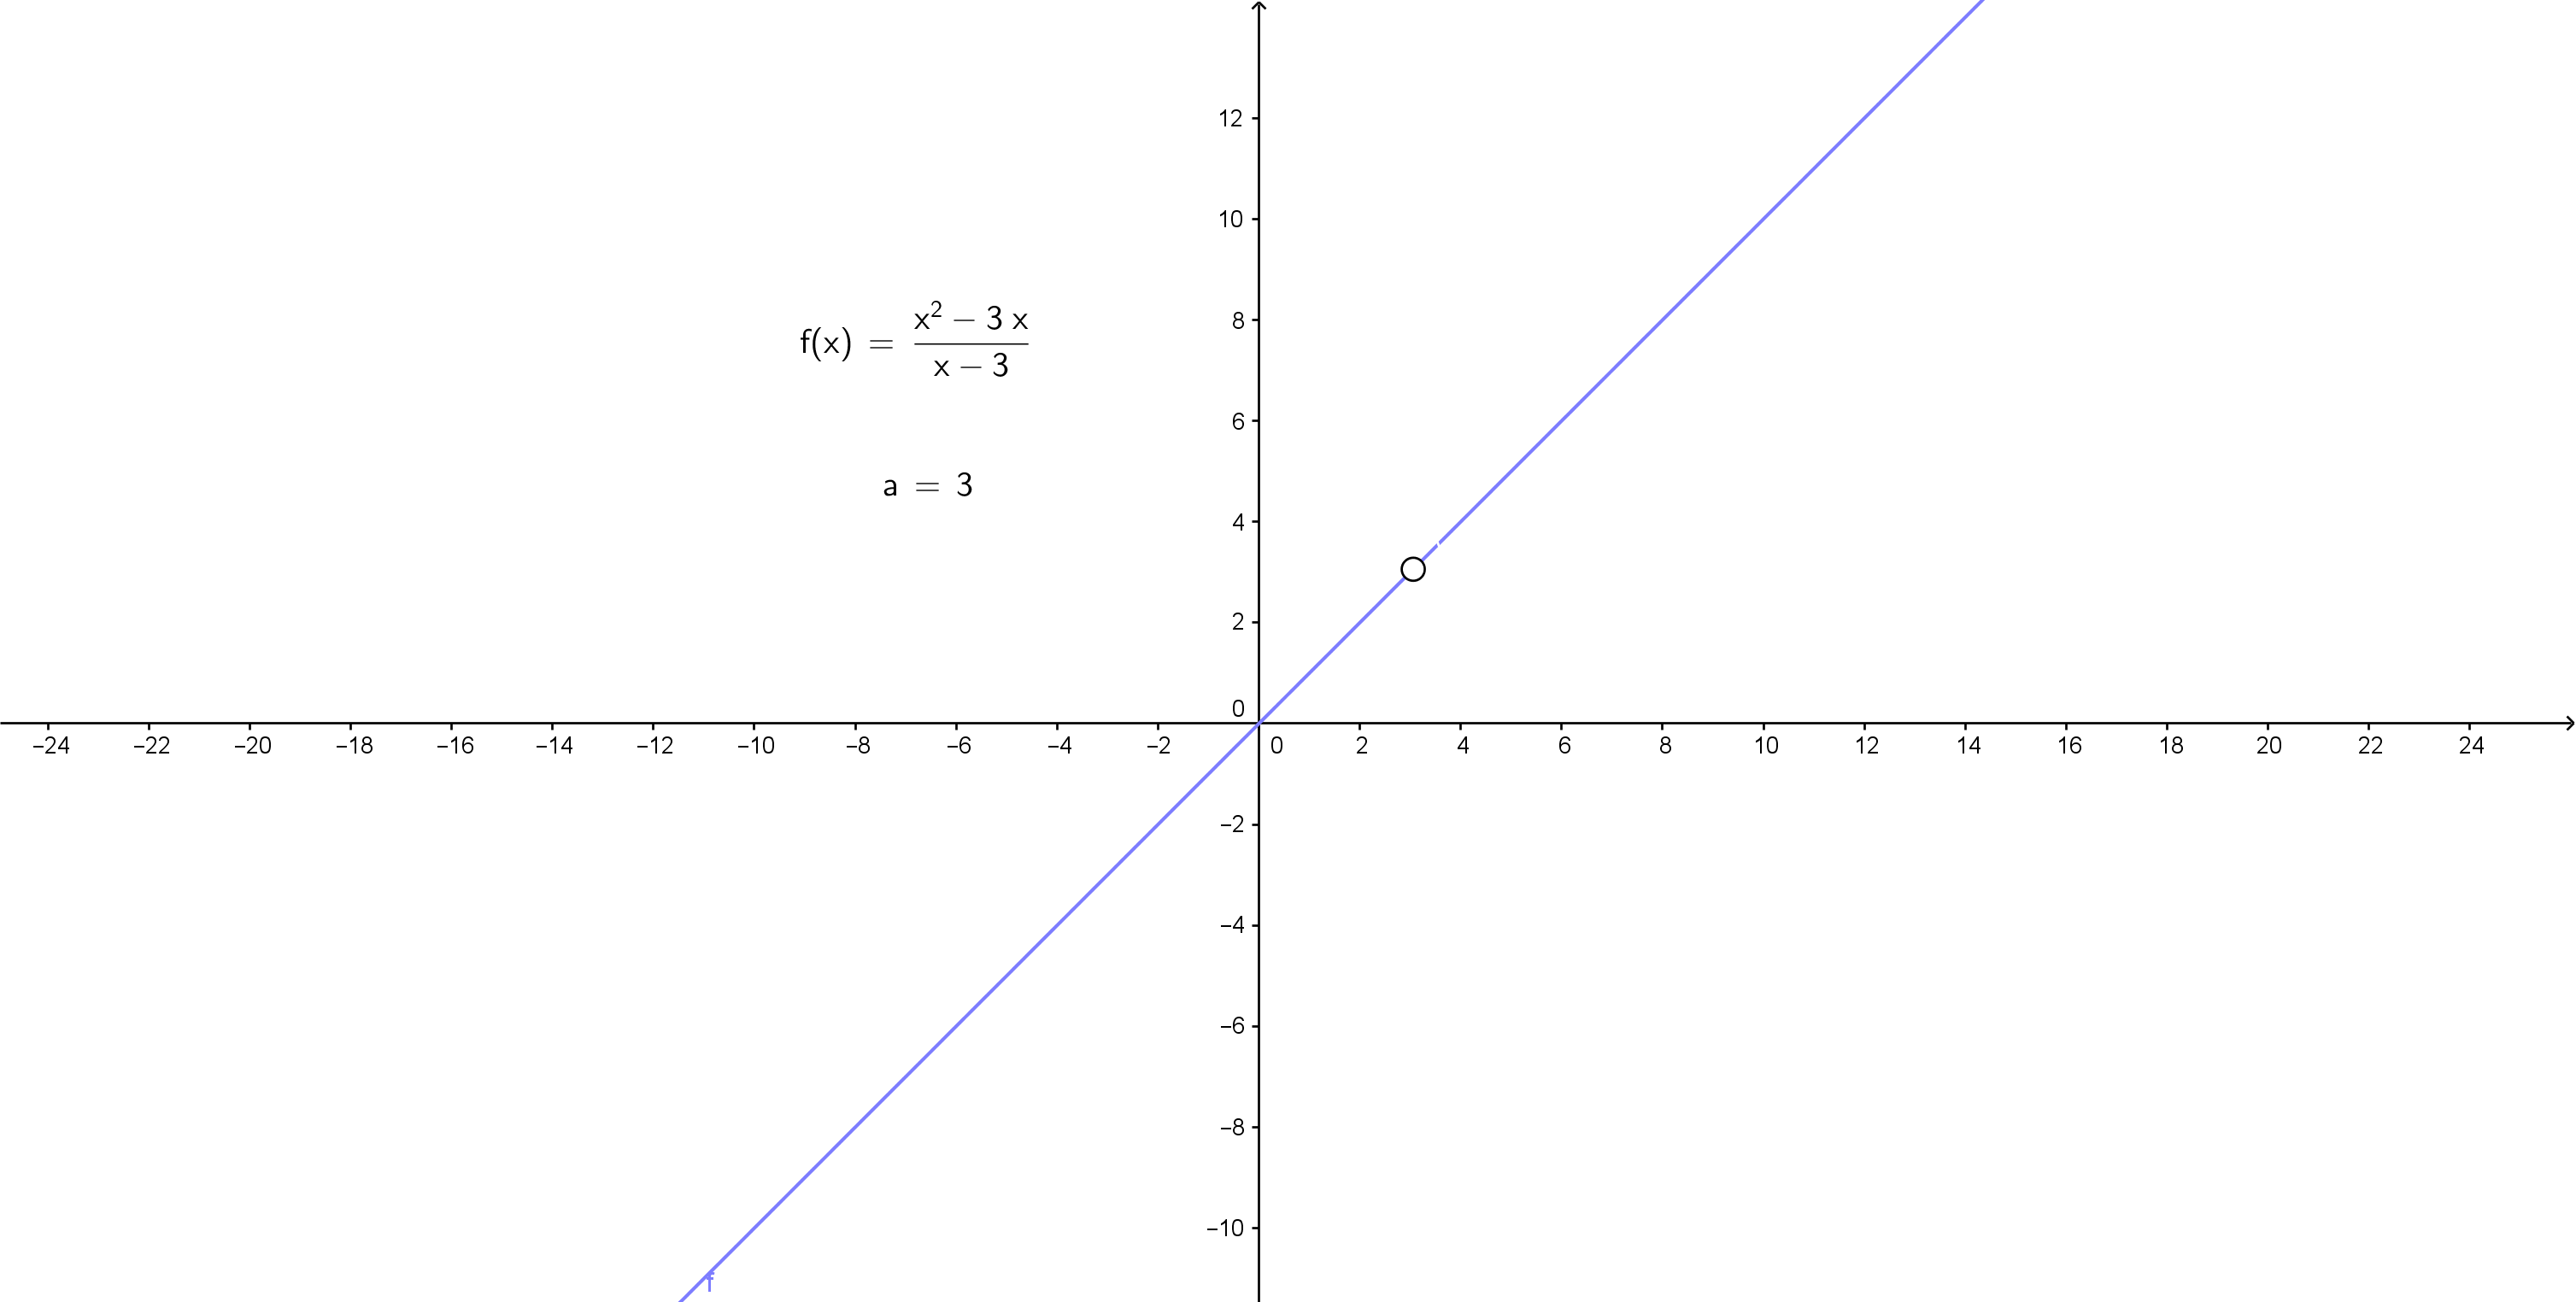
\includegraphics[width=15cm]{img/graph7.png} % leia abaixo
\caption{Gráfico de $f(x)$}
\label{fig:graph7}
\end{figure}

\textbf{Teorema 4}
(Teorema do confronto). Segundo \citeonline[p.110 ]{stewart} \textit{Se $f(x) \leq g(x) \leq h(x)$ quando $x$ está próximo de $a$ (exceto possivelmente em $a$), e 
$$
\lim_{x \to a} f(x) = \lim_{x \to a} h(x) = L
$$
então
$$
\lim_{x \to a} g(x) = L
$$
}\\

\textbf{Exemplo 3} Limite fundamental trigonométrico $\displaystyle \lim_{x \to 0} \frac{sen(x)}{x}$\\ 

Atribuindo valores a $x$ pela direita e pela esquerda de zero, conforme mostra a tabela \ref{tab:sen}, notamos que, para valores cada vez mais próximos de zero, obtem-se valores de $\displaystyle f(x) = \frac{sen(x)}{x}$  cada vez mais próximos de 1.

\begin{table}[H]
\centering
\caption{Tabela de valores para $\displaystyle \frac{sen(x)}{x}$}
\label{tab:sen}
\smallskip
\begin{tabular}{l|l}
\hline
&\\[-2ex]
 $x$ & $\displaystyle \frac{sen(x)}{x}$ \\[0.5ex]
\hline
&\\[-2ex]
$\displaystyle \pm 1$ & $0,84147098$ \\[0.5ex]
\hline
&\\[-2ex]
$\pm 0,5$ & $0,95885108$ \\[0.5ex]
\hline
&\\[-2ex]
$\pm 0,4$ & $0,97354586$ \\[0.5ex]
\hline
&\\[-2ex]
$\pm 0,3$ & $0,98506736$ \\[0.5ex]
\hline
&\\[-2ex]
$\pm 0,2$ & $0,99334665$ \\[0.5ex]
\hline
&\\[-2ex]
$\pm 0,1$ & $0,99833417$ \\[0.5ex]
\hline
&\\[-2ex]
$\pm 0,05$ & $0,99958339$ \\[0.5ex]
\hline
&\\[-2ex]
$\pm 0,01$ & $0,99998333$ \\[0.5ex]
\hline
&\\[-2ex]
$\pm 0,005$ & $0,99999583$ \\[0.5ex]
\hline
&\\[-2ex]
$\pm 0,001$ & $0,99999983$ \\[0.5ex]
\hline
\end{tabular}
\end{table}

Assim, tem-se $\displaystyle \lim_{x \to 0} \frac{sen(x)}{x} = 1$\\
\begin{figure}[H]
\centering % para centralizarmos a figura
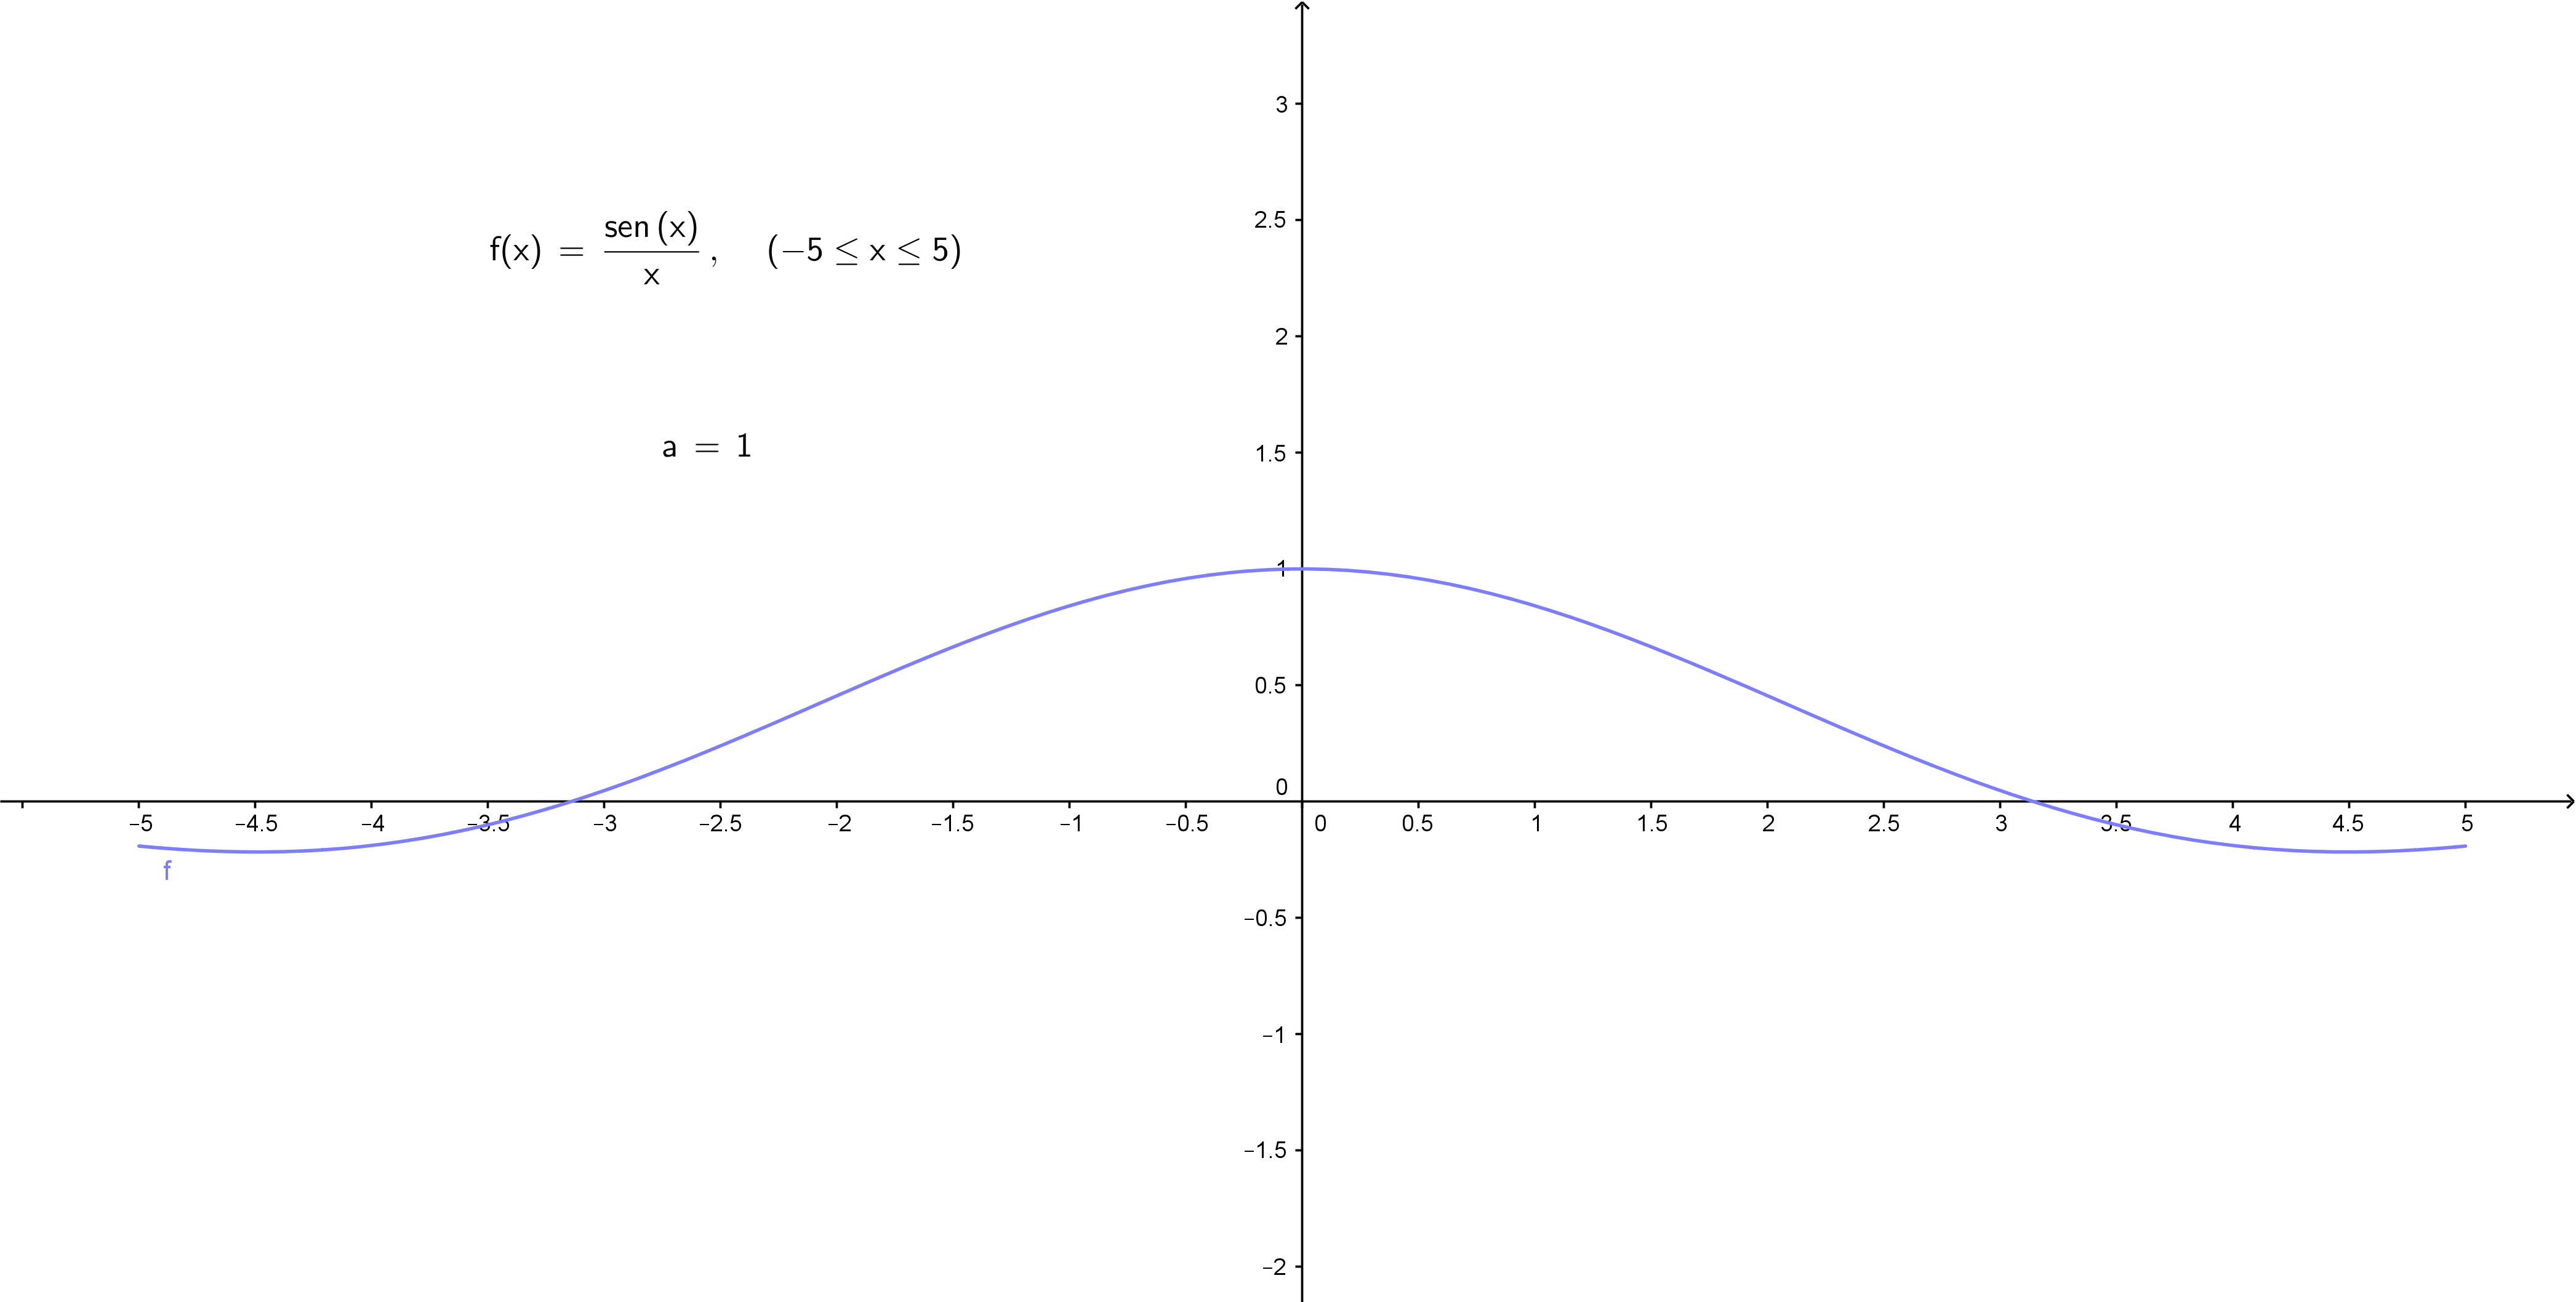
\includegraphics[width=15cm]{img/graph8.png} % leia abaixo
\caption{Gráfico de $f(x)$.}
\label{fig:graph8}
\end{figure}
Demonstração: Cosiderando a circunferência de raio 1.
\begin{figure}[H]
\centering % para centralizarmos a figura
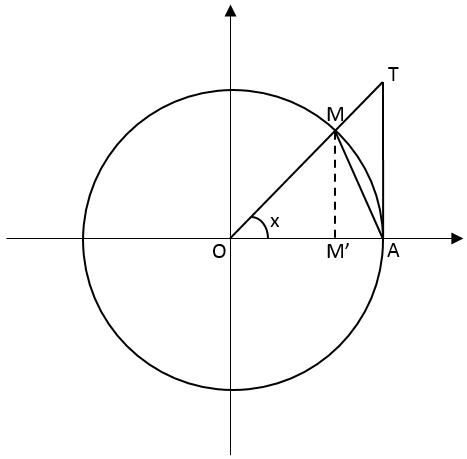
\includegraphics[width=10cm]{img/img1.png} % leia abaixo
\caption{Circunferência de raio 1}
\label{fig:circ1}
\end{figure}

Seja $x$ a medida em radianos do arco ${AOM}$ e considerando $x$ entre 0 e $\displaystyle \frac{\pi}{2}$ de acordo com a Figura \ref{fig:circ1}. Observa-se que:
$$
\textrm{área} \bigtriangleup MOA <  \textrm{área setor $MOA$}  < \textrm{área $\bigtriangleup  AOT$}
$$
$$
\frac{OA.MM}{2} < \frac{OA . AM}{2} < \frac{OA . AT}{2}
$$
$$
MM' < AM < AT
$$
$$
sen (x) < x < tg(x)
$$

Dividindo tudo por $sen(x) > 0$, vem:\\
\begin{equation}
\label{eq:dem1}
\frac{sen(x)}{sen(x)} < \frac{x}{sen(x)} < \frac{tg(x)}{sen(x)} = \begin{tabular}{|p{4.0cm}|} \hline  $\displaystyle 1 < \frac{x}{sen(x)} < \frac{tg(x)}{sen(x)}$\\ \hline \end{tabular}
\end{equation}\\




Sendo: $\displaystyle tg(x) = \frac{sen(x)}{cos(x)}$, então, $$\displaystyle \frac{tg(x)}{sen(x)} = \frac{\frac{sen(x)}{cos(x)}}{sen(x)} = \frac{sen(x)}{sen(x)} . \frac{1}{cos(x)} = \frac{1}{cos(x)}$$ Substituindo em \ref{eq:dem1}, tem-se:
$$
1 < \frac{x}{sen(x)} < \frac{1}{cos(x)} \quad \textrm{, invertendo obtem-se:}\\
1 > \frac{sen(x)}{x} > cos(x)
$$
Como o $\displaystyle \lim_{x \to 0} (1) = 1$ e $\displaystyle \lim_{x \to 0} cos(x) = cos(0) = 1$, então de acordo com o teorema do confronto a função $\displaystyle \frac{sen(x)}{x}$, que esta entre $cos(x)$ e $1$, tem também limite igual a $1$ quando $x$ tende a $0$ (zero), logo:
$$
\lim_{x \to 0} \frac{sen(x)}{x} = 1
$$


\subsection{Forma do Tipo $\displaystyle \frac{\infty}{\infty}$}
Esta forma de indeterminação ocorre quando se tem no numerador e no denominador polinômios com $x \to \pm \infty$.\\


\textbf{Exemplo 1}$$\displaystyle \lim_{x \to \infty} f(x) = \lim_{x \to \infty} \frac{2x^5+3x+5}{4x^3 -2} = \frac{2 . \infty^5 + 3 . \infty + 5}{4 . \infty^3 -2} = \frac{\infty}{\infty}$$\\

Para solucionar a indeterminação precisa-se manipular algebricamente a expressão.\\

\quad Conforme \citeonline[p. 101]{guidorizzi}i, coloca-se em evidência a mais alta potência de $x$ que ocorre no numerador e procede-se da mesma forma no denominador. Deste modo, irão aparecer no denominador e numerador expressões do tipo $\displaystyle \frac{1}{x^n}$ que tendem a zero para $x \to + \infty$, o que facilitará o cálculo do limite.
$$
\lim_{x \to \infty}  \frac{2x^5+3x+5}{4x^3 -2} =  \lim_{x \to \infty} \frac{x^5(2+\frac{3}{x^4} + \frac{5}{x^5})}{x^3(4-\frac{2}{x^3})} = \lim_{x \to \infty} \frac{2x^5}{x^3} = \lim_{x \to \infty} 2x^2 = 2. \infty^2 = + \infty
$$



\begin{figure}[H]
\centering % para centralizarmos a figura
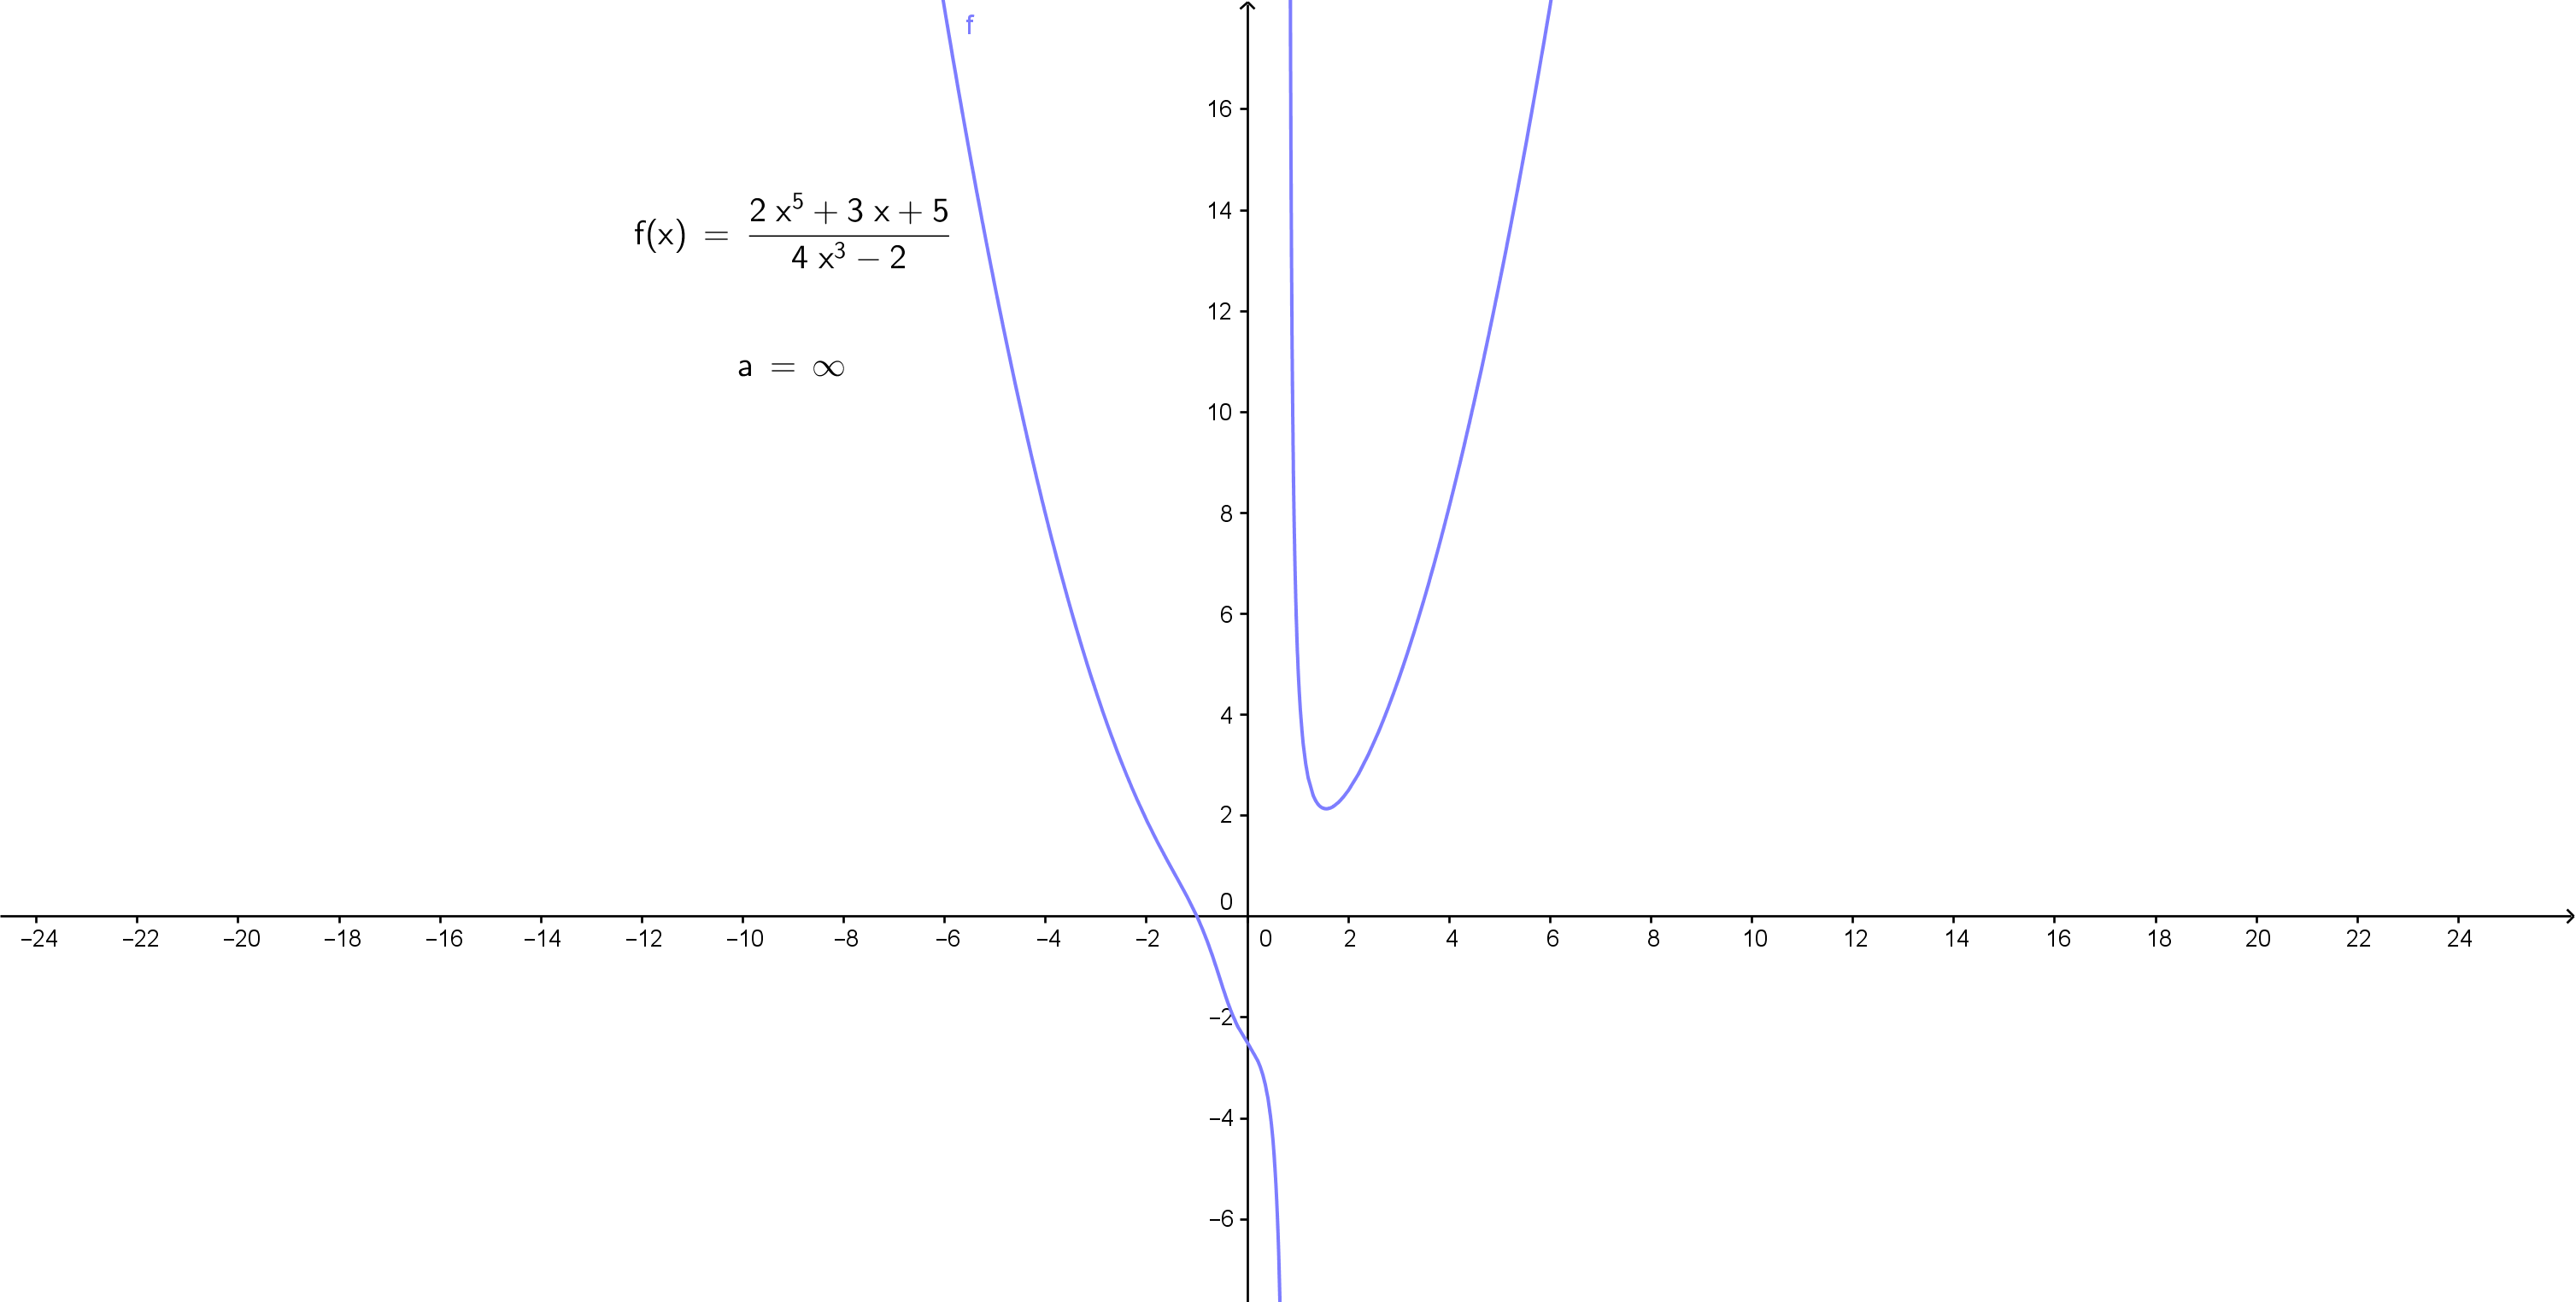
\includegraphics[width=15cm]{img/graph9.png} % leia abaixo
\caption{Gráfico de $ f(x)$}
\label{fig:graph9}
\end{figure}

Observa-se que se o grau do numerador for superior ao grau do denominador então o limite é mais ou menos infinito.\\
 

\textbf{Exemplo 2} $$\displaystyle  \lim_{x \to \infty}f(x) = \lim_{x \to \infty} \frac{5x^4}{2x^3} = \lim_{x \to \infty} \frac{5 \infty^4}{2 \infty^5} = \frac{\infty}{\infty} \quad \textrm{Indeterminação}$$\\
Para solucionar esta indeterminação deve-se simplificar a expressão dividindo tudo por $x^3$.
$$
\lim_{x \to \infty}f(x) = \lim_{x \to \infty} \frac{5x^4}{2x^3} = \lim_{x \to \infty} \frac{\frac{5x^4}{x^3}}{\frac{2x^3}{x^3}} = \lim_{x \to \infty} \frac{5x}{2} = \infty
$$

Observa-se que o comportamento do polinômio no infinito é ditado pelo termo de maior grau, chamado de termo dominante.\\
\begin{figure}[H]
\centering % para centralizarmos a figura
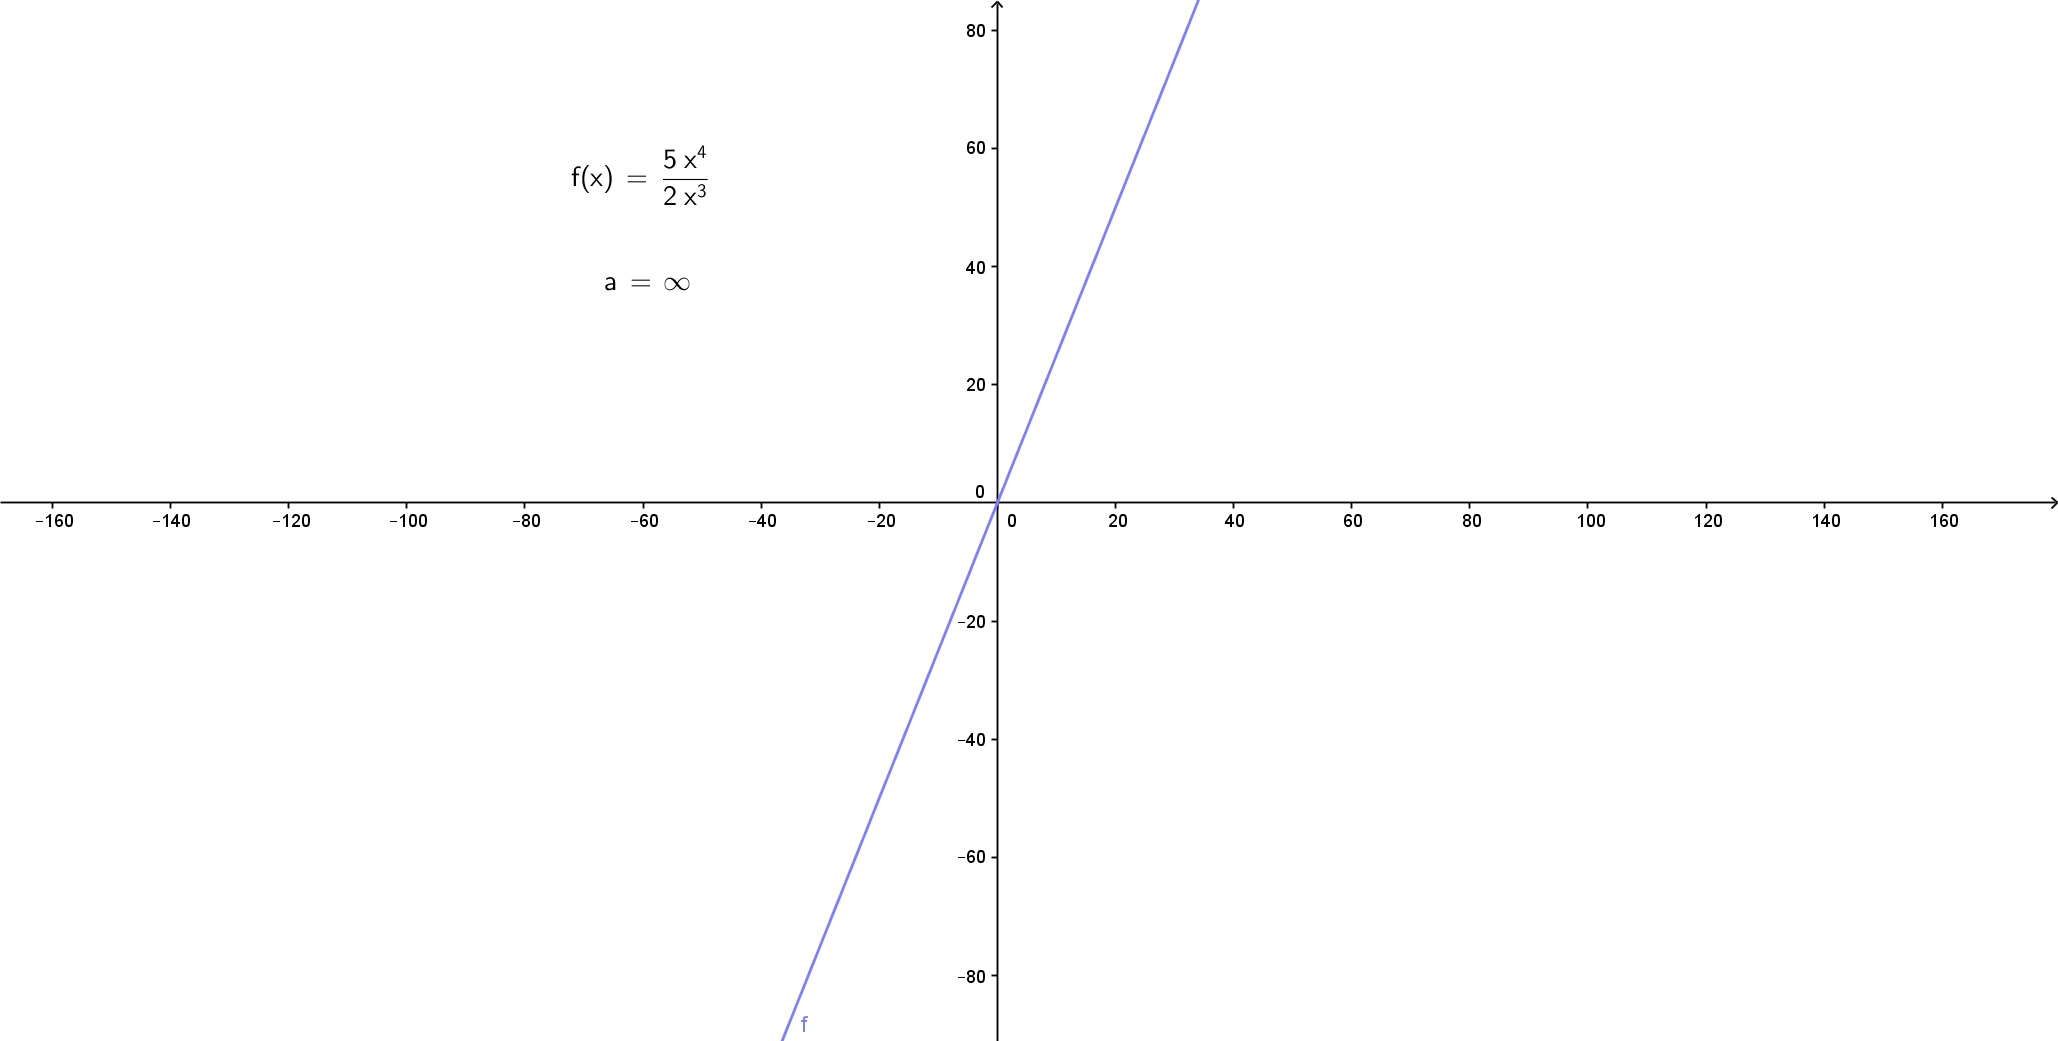
\includegraphics[width=15cm]{img/graph10.png} % leia abaixo
\caption{Gráfico de $f(x)$}
\label{fig:graph10}
\end{figure}

\textbf{Exemplo 3}
$$
\lim_{x \to +\infty} f(x) = \lim_{x \to +\infty} \frac{x^2+2x+3}{x^2+x} = \frac{\infty^2+2\infty+3}{\infty^2+\infty}= \frac{\infty}{\infty}
$$\\
Para solucionar esta indeterminação coloca-se o $x^2$ em evidência, logo:
$$
\lim_{x \to +\infty} \frac{x^2(1+\frac{2}{x}+\frac{3}{x^2})}{x^2(1+\frac{1}{x})} = \lim_{x \to +\infty} \frac{x^2}{x^2}= \lim_{x \to +\infty} \frac{1}{1} = 1
$$
Observa-se que quando se tem uma função polinominal com numerador e denominador do mesmo grau, o limite é o quociente dos coeficientes dos termos de maior grau.\\
\begin{figure}[H]
\centering % para centralizarmos a figura
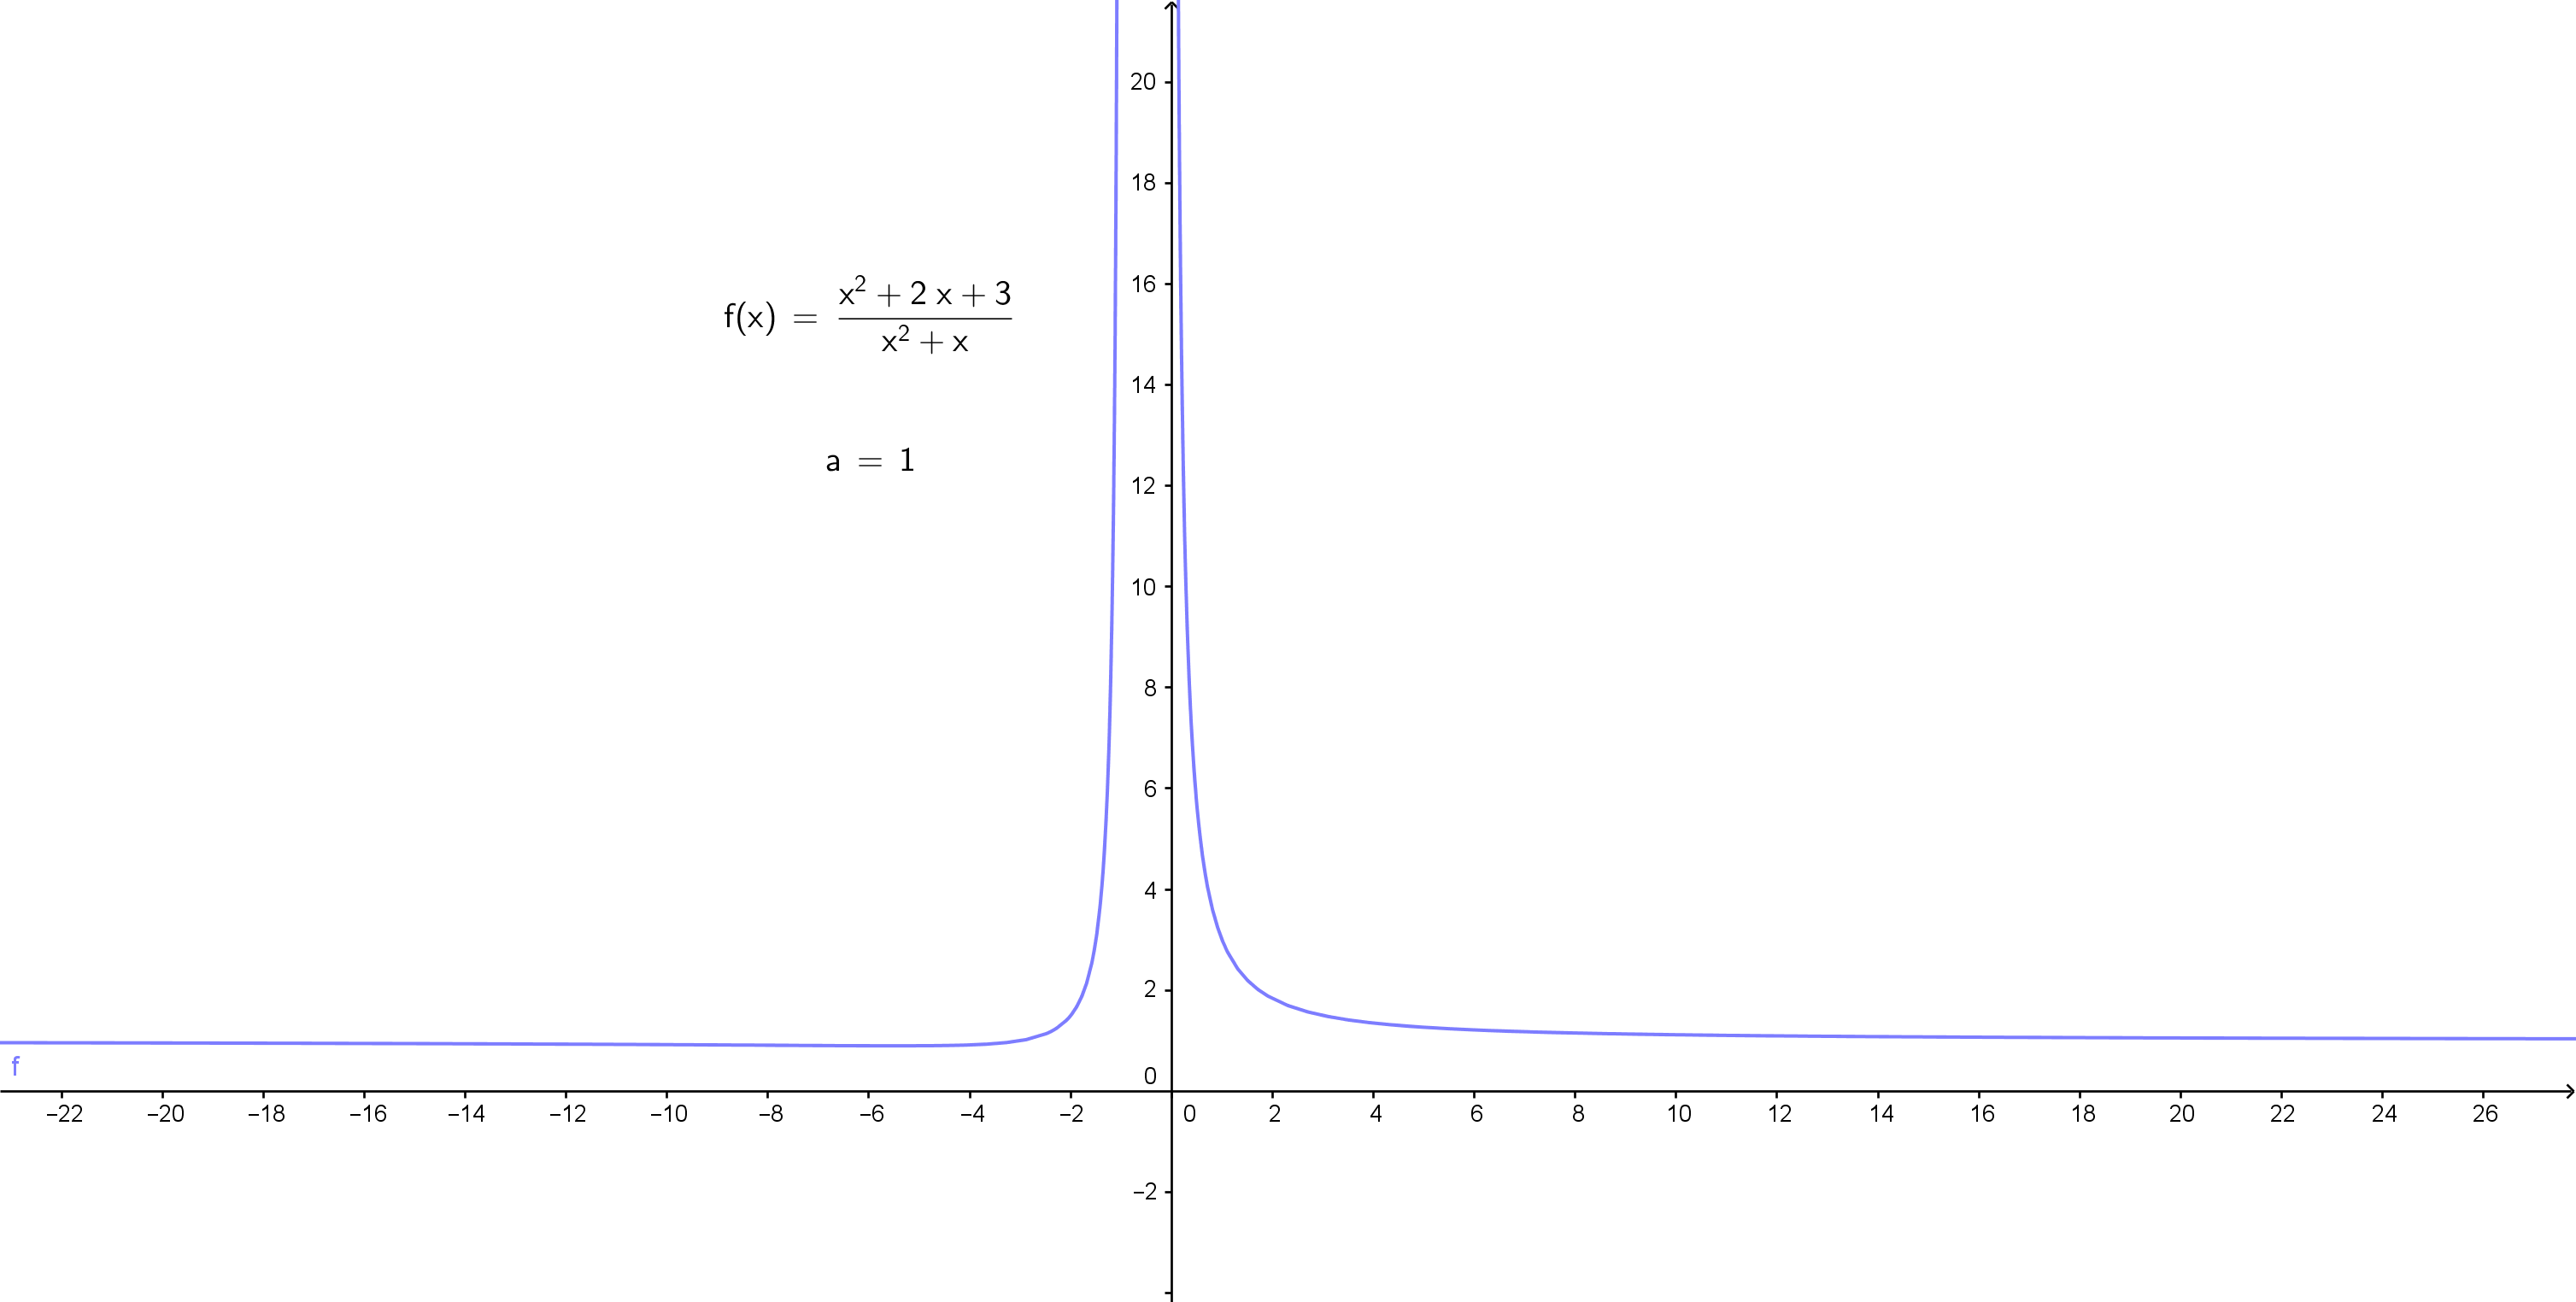
\includegraphics[width=15cm]{img/graph11.png} % leia abaixo
\caption{Gráfico de $f(x)$}
\label{fig:graph11}
\end{figure}

\textbf{Teorema 5}
(Limites infinitos com $x \to \pm \infty$) Segundo \citeonline[p. 90]{leithold}\textit{ Se $r$ for um inteiro positivo qualquer, então:\\
i) $\displaystyle \lim_{x \to + \infty} \frac{1}{x^r} = 0$\\
ii) $\displaystyle \lim_{x \to - \infty} \frac{1}{x^r} = 0$}\\


\textbf{Exemplo 4} $$\displaystyle \lim_{x \to \infty} f(x) = \lim_{x \to \infty} \frac{2x^3-3x+2}{4x^4-5} = \frac{\infty}{\infty} \quad \textrm{indeterminado}$$\\
Para solucionar a indeterminação $\displaystyle \frac{\infty}{\infty}$ divide-se todos os termos pelo termo de maior grau, obtendo:
$$
\lim_{x \to \infty} \frac{\frac{2x^3}{x^4} - \frac{3x}{x^4}+\frac{2}{x^4}}{\frac{4x^4}{x^4} - \frac{5}{x^4}} = \lim_{x \to \infty} \frac{0}{4} = 0
$$ 

Observa-se que quando o grau do numerador for inferior ao grau do denominador o limite será zero para $x$ tendendo ao infinito.\\
\begin{figure}[H]
\centering % para centralizarmos a figura
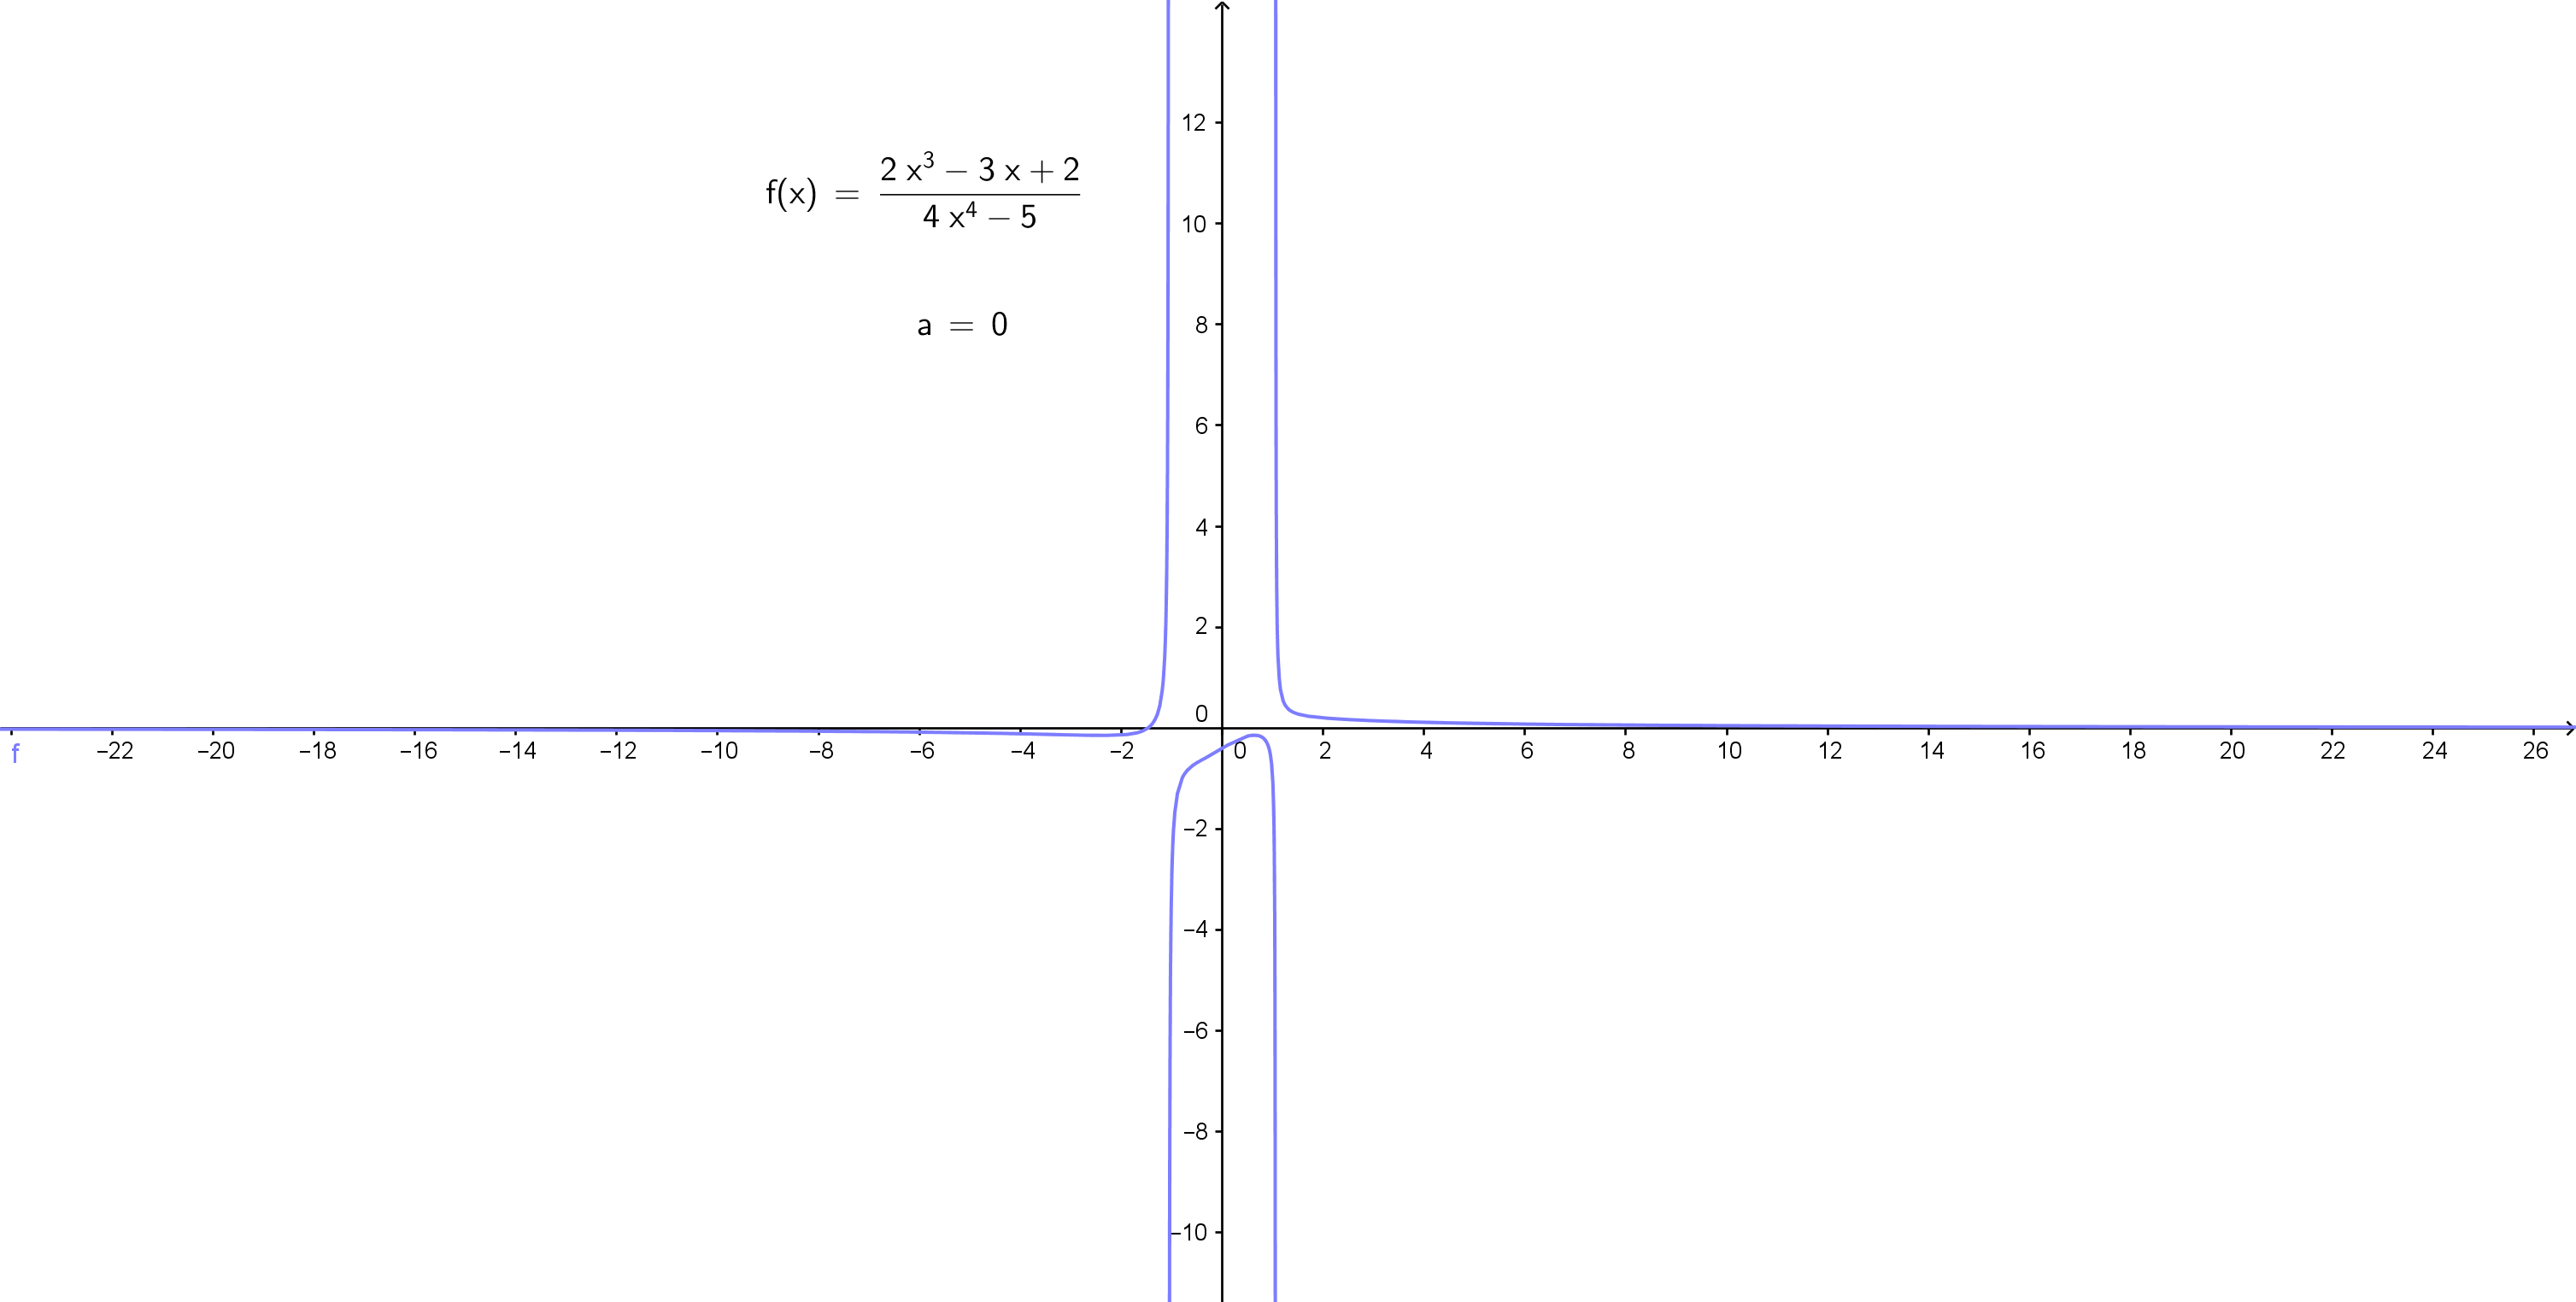
\includegraphics[width=15cm]{img/graph12.png} % leia abaixo
\caption{Gráfico de $f(x)$}
\label{fig:graph12}
\end{figure}



\subsection{Forma do Tipo $\infty - \infty$}
\quad Primeiramente, vale lembrar que pode acontecer que a diferença entre $f$ e $g$ quando duas funções tendem ao infinito, que o limite pode ser finito, como por exemplo:\\

Seja $\displaystyle f(x) = K + \frac{1}{x}$ e $\displaystyle g(x) = \frac{1}{x}$, onde $K$ é uma constante arbitrária. Logo,
$$
\lim_{x \to 0} f(x) = \lim_{x \to 0} g(x) = \infty
$$
$$
\lim_{x \to 0} [f(x) - g(x)] = K
$$

Esse exemplo mostra que é possível um limite da forma do tipo $\infty - \infty$ ter limite finito. Entretanto limite dessa forma também pode ser infinito.\\


\textbf{Exemplo 1} Seja $\displaystyle \lim_{x \to \infty}f(x) = \lim_{x \to \infty} (x^3-3x^2) = \lim_{x \to \infty} x^3 - \lim_{x \to \infty} 3x^2 = \infty - \infty$\\
Logo, não podemos aplicar a Lei do Limite, pois $\infty$ não é  um número (não se pode definir $\infty - \infty$). No entanto, pode-se escrever:
$$
\lim_{x \to \infty} (x^3-3x^2) = \lim_{x \to \infty} x^2(x-3) = \infty
$$
pois, como $x^2$ e $x-3$ tornam-se arbitrariamente grandes, o mesmo acontece com seu produto.

\begin{figure}[H]
\centering % para centralizarmos a figura
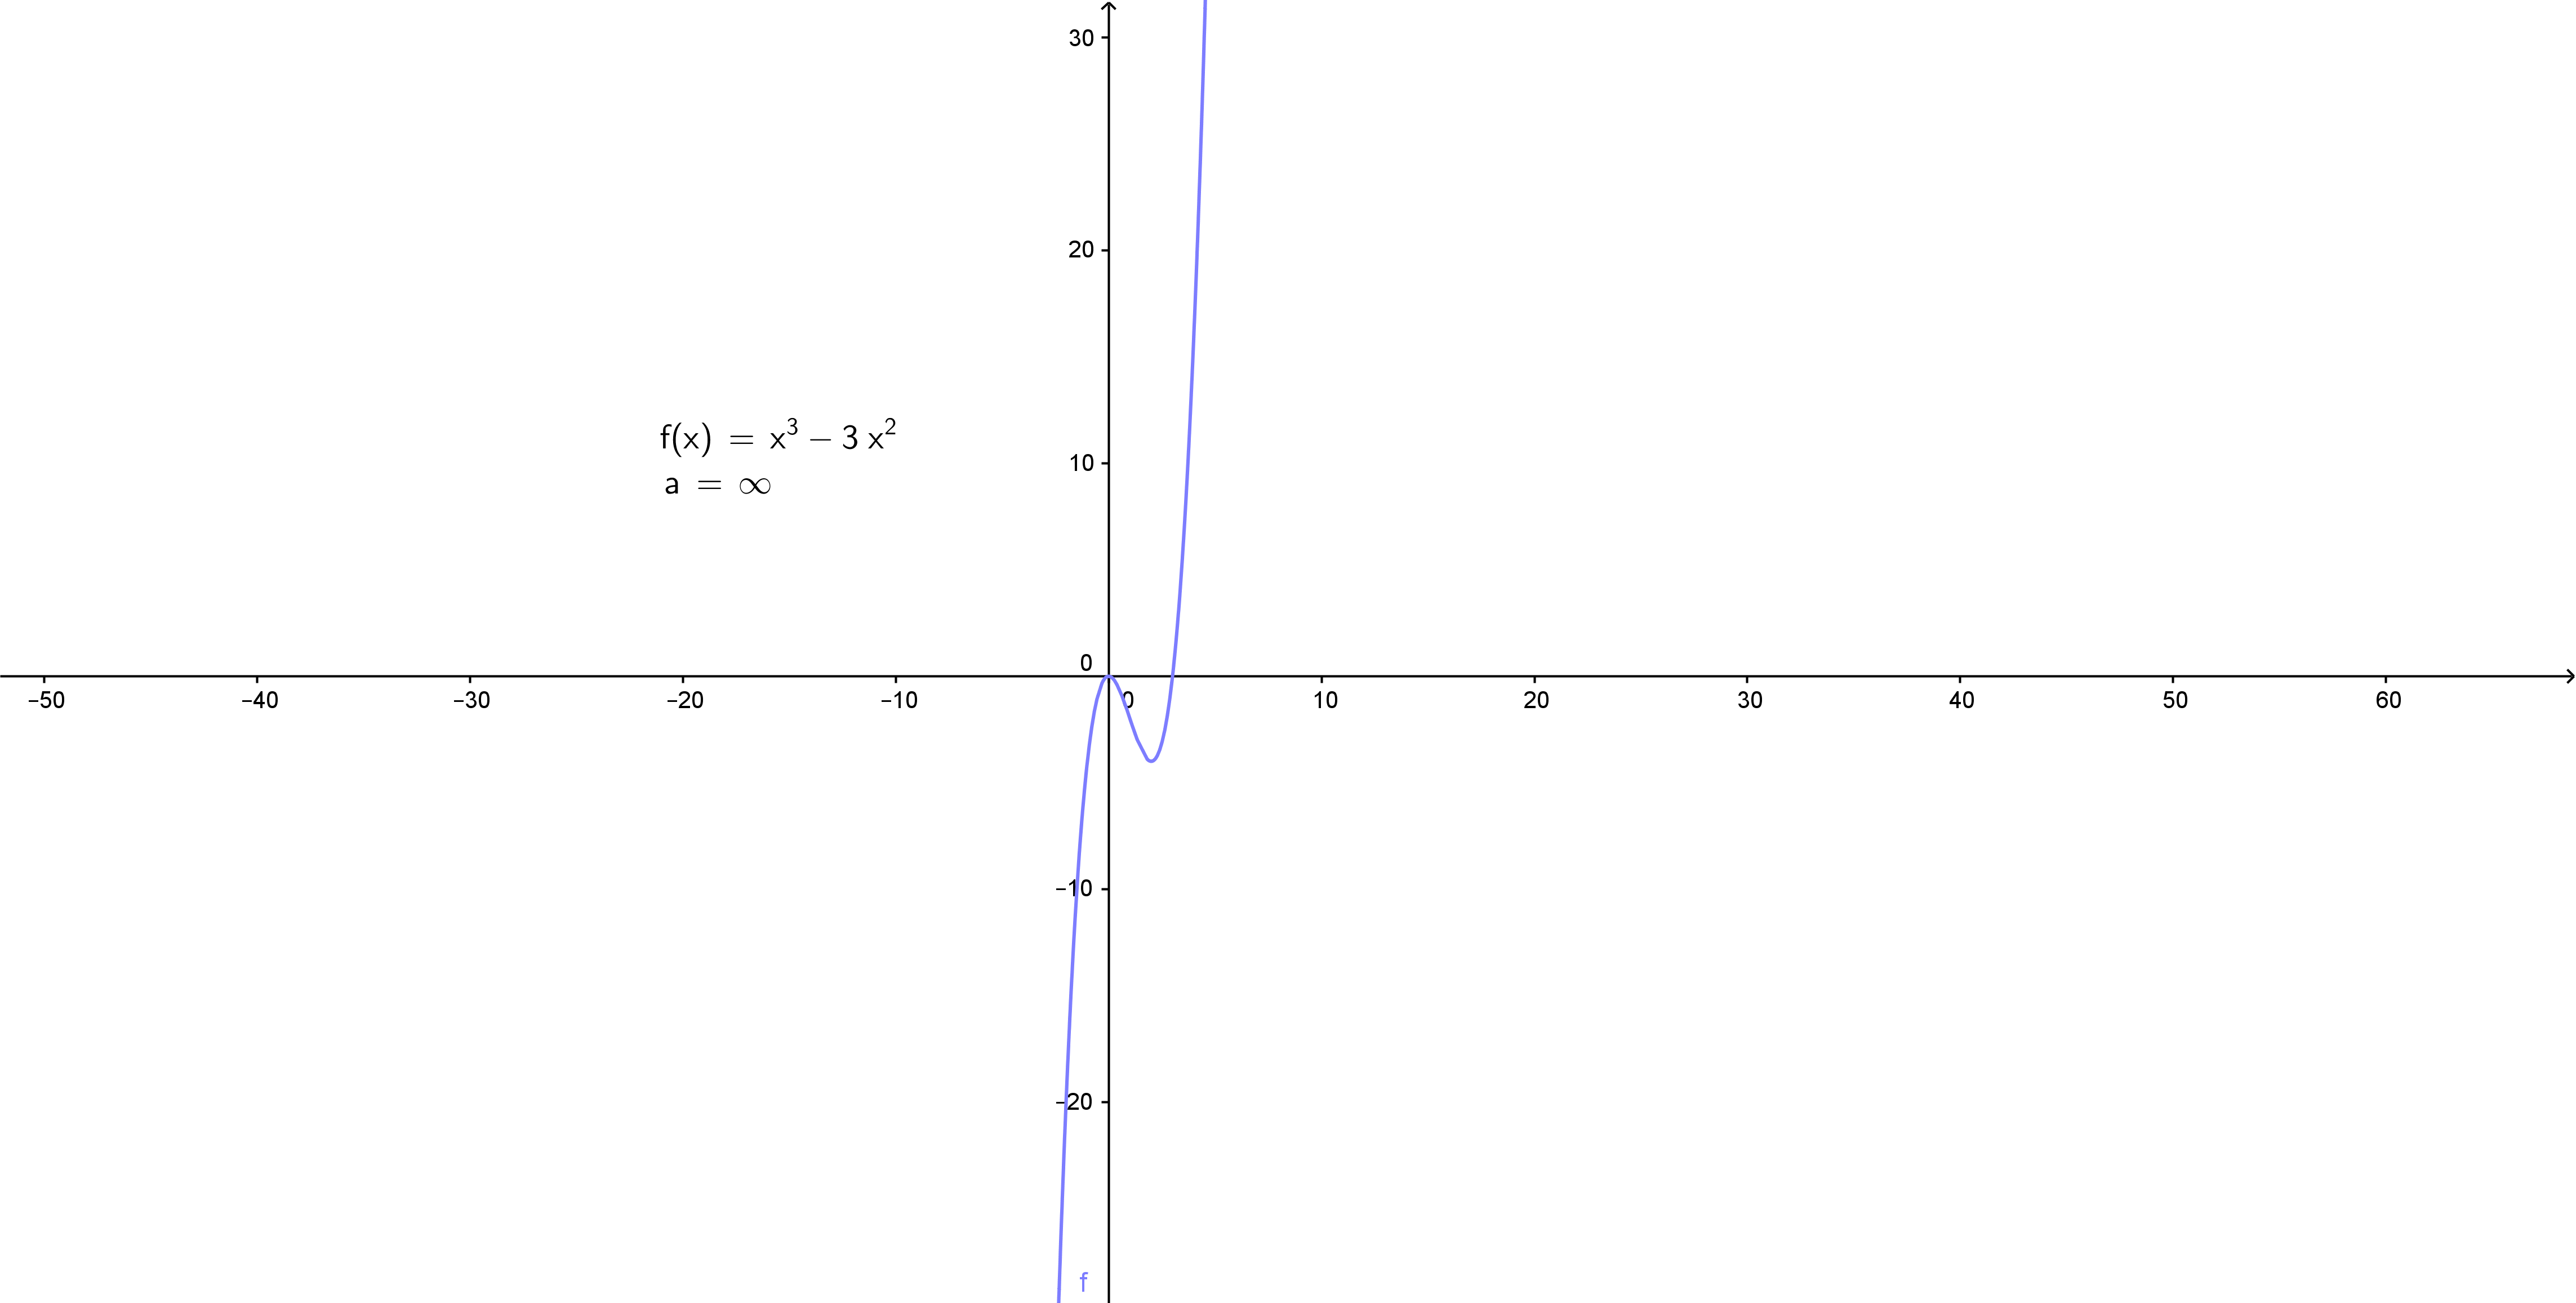
\includegraphics[width=15cm]{img/graph13.png} % leia abaixo
\caption{Gráfico de $f(x)$}
\label{fig:graph13}
\end{figure}


\textbf{Exemplo 2} $$\displaystyle \lim_{x \to +\infty}f(x) = \lim_{x \to +\infty} (x^3-2x^2+3) = \infty - \infty$$\\
Para solucionar a indeterminação utiliza-se artificios do cálculo, colocando $x^3$ em evidência.
$$
\lim_{x \to + \infty}f(x) = \lim_{x \to + \infty} (x^3-2x^2+3)
$$\\
$$
\lim_{x \to \infty} x^3(1-\frac{2}{x}+\frac{3}{x^3}) = \lim_{x \to \infty} x^3 = + \infty
$$
\begin{figure}[H]
\centering % para centralizarmos a figura
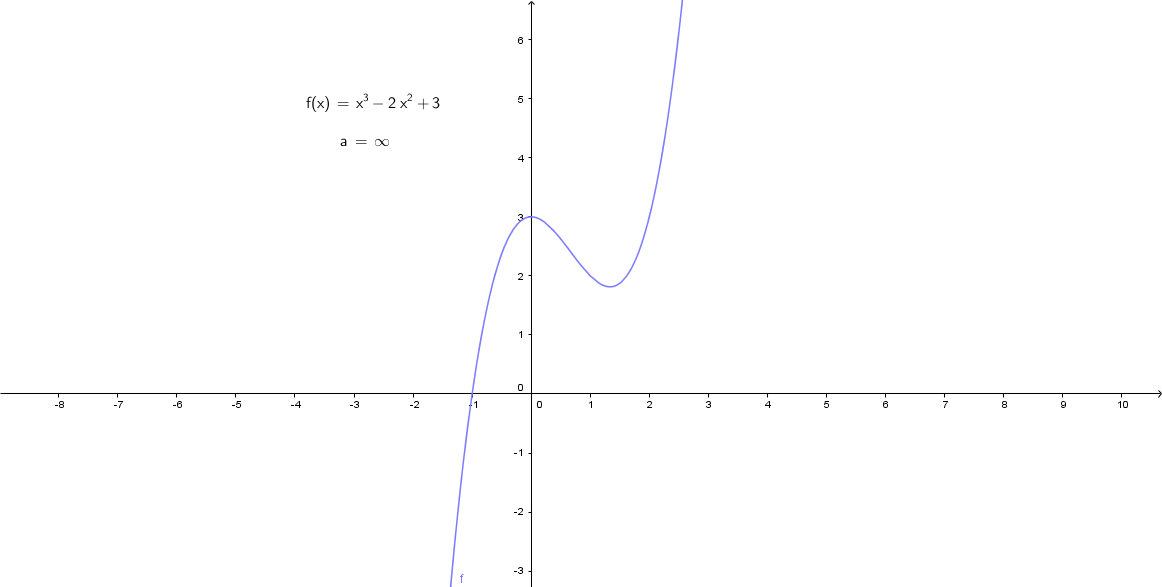
\includegraphics[width=15cm]{img/graph14.png} % leia abaixo
\caption{Gráfico de $ f(x)$}
\label{fig:graph14}
\end{figure}

\section{Forma Indeterminada do tipo $0.\infty$}
A indeterminação $0.\infty$ pode ser tranformada numa indeterminação do tipo $\displaystyle \frac{\infty}{\infty}$ ou $\displaystyle \frac{0}{0}$, vejamos:\\

\textbf{Exemplo 1}
$$
\lim_{x \to \infty} f(x) = \lim_{x \to \infty} (x+7)\sqrt{\frac{1}{4x^2+3}} = \infty . 0
$$ 
$$
\lim_{x \to \infty} (x+7)\sqrt{\frac{1}{4x^2+3}} = \lim_{x \to \infty} \sqrt{\frac{(x+7)^2}{4x^2+3}} = \frac{\infty}{\infty} = \lim_{x \to \infty} \sqrt{\frac{x^2+14x+49}{4x^2+3}}
$$
Como visto no exemplo 3 com funções polinomiais de mesmo grau, tem-se que o limite é o quocientes dos coeficientes dos termos de maior grau, logo:
$$
\lim_{x \to \infty} \sqrt{\frac{x^2+14x+49}{4x^2+3}} = \lim_{x \to \infty} \sqrt{\frac{1}{4}} = \frac{1}{2}
$$

\begin{figure}[H]
\centering % para centralizarmos a figura
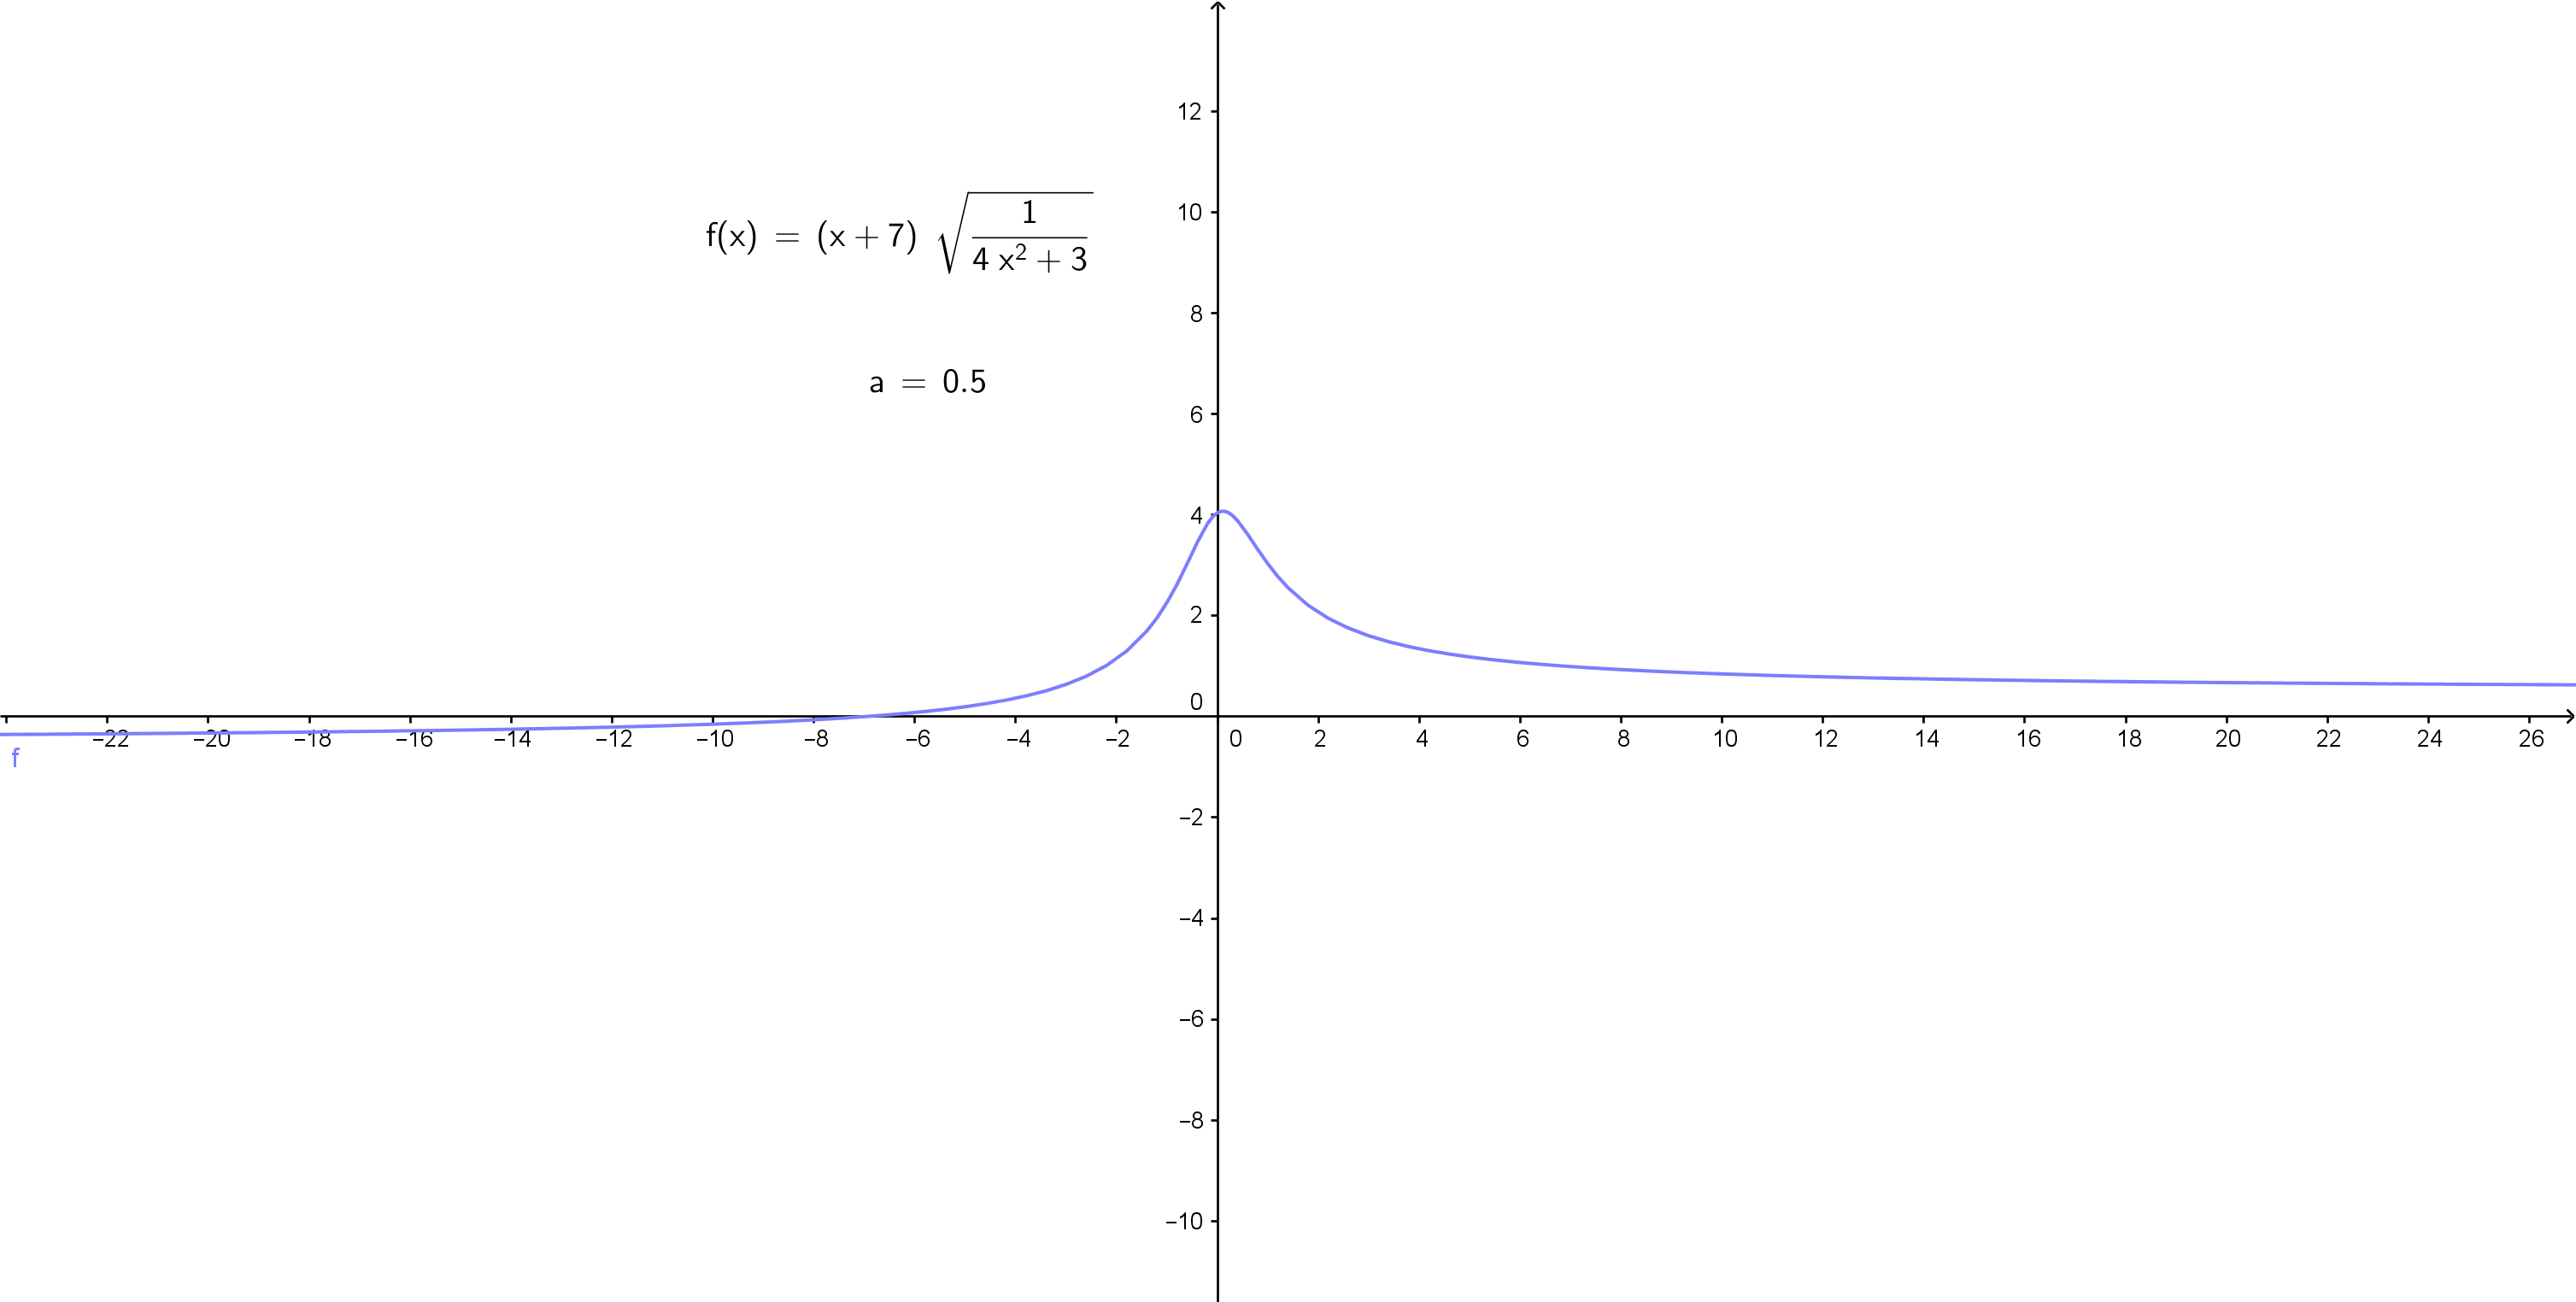
\includegraphics[width=15cm]{img/graph15.png} % leia abaixo
\caption{Gráfico de $f(x)$}
\label{fig:graph15}
\end{figure}

\textbf{Exemplo 2}
$$
\lim_{x \to 0} f(x) = \lim_{x \to 0} x . \frac{1}{4x} = \frac{0}{0}
$$
simplificando, temos:
$$
\lim_{x \to 0} \frac{1}{4} = \frac{1}{4}
$$

Lembrando que a função não está definida para $x$ igual a zero, apenas nas proximidades de zero, logo pela definição de limite se permite dividir o numerador e o denominador por $x$.
\begin{figure}[H]
\centering % para centralizarmos a figura
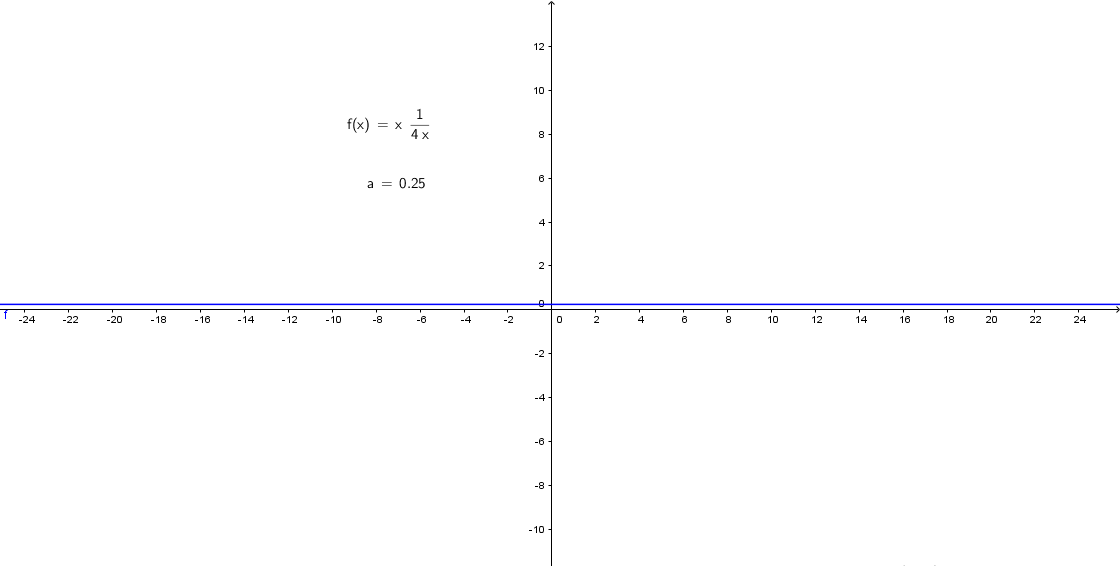
\includegraphics[width=15cm]{img/sub2.png} % leia abaixo
\caption{Gráfico de $f(x)$}
\label{fig:graph1}
\end{figure}
\quad Observa-se que os casos de indeterminações foram resolvidos através do uso de técnicas matemáticas, porém existe outro método para resolvê-los, conhecido como Regra de L'Hôspital, a qual não explanaremos neste trabalho. 































 